\chapter{Combined search for invisibly decaying Higgs bosons in hadronic channels}
\label{chap:higgstoinv}

\epigraph{Invisibility---there are things we can't see now, that are there, that are embedded, that it really takes time in order to be able to see. There are many ghosts that are lurking around and lingering through us that takes the technology of another generation or so in order to uncover and show what those stains and strains and perceived flaws really we're building towards.}{--- Lynn Hershman Leeson}

\initial{P}articles that escape the detector unseen in any experiment make them, by design, notoriously difficult to search for. The Higgs boson is particularly troublesome with its small production rate at the \acrshort{lhc} and a commensurate prediction of the invisible state branching ratio. As described in Chpt.~\ref{sec:theory_higgs_to_inv}, the leading estimates are still far higher than the \acrlong{sm}'s value. For the best chance of observing this decay, the inclusion of all of the Higgs boson's production modes is a necessity.

%=======
\begin{easylist}[itemize]
    \easylistprops
    & Emphasize my contributions: control region construction and studies, background estimation, ttbar systematics, and other studies I will have conducted by the time I write up (check AN, chip and HToInv-nanoAOD-tools MRs, and git commit history).

    & Maintaining CMS internal analysis note, documenting all aspects of the analysis. I will first add all relevant information there which I can subsequently use when writing this chapter.

    & Since it's my thesis, I can talk about \ttH, \VH and \ggH, even though the Bristol contribution to the final, public result may only be \ttH and resolved \VH. Would need to be able to run the fit for all three modes simultaneously, ensuring we have complete (and correct) systematics for \ggH.
\end{easylist}

% Can pull from Section 37 of my lab book, and all the talks I and other people from the team have given (Presentations and talks/ folder, also Other peoples/ subdirectory). Can also pull from AN for analysis strategy


%=========================================================


\import{./}{overview_software.tex}


%=========================================================


\import{./}{data_simulation.tex}


%=========================================================


\import{./}{event_selection.tex}


%=========================================================


\import{./}{categorisation.tex}


%=========================================================


\import{./}{region_definitions.tex}


%=========================================================


\import{./}{background_estimation.tex}


%=========================================================


\import{./}{weights_and_systs.tex}


%=========================================================


\section{Statistical model and fit}
\label{sec:htoinv_satistical_treatment}

% Give an outline of the how the fit is done (likelihood model, writing it out in full and highlighting each aspect) and how the background estimation methods factor in, etc. Like background estimation, describe it generally since I didn't explicitly work on it. Current fit model is given at https://indico.cern.ch/event/934008/contributions/3924639/attachments/2065231/3465892/2020_06_15_CHIP_Meeting_nonVBF_fit.pdf

% In the following sections, talk more about the specific aspects for each mode (e.g., dropping dilepton CRs for ttH, using photon CR only for VH)

% Toys (verbatim from Henning): toys are repeat experiments where you draw new values for your observed signal and bg based on the uncertainties associated with both. The parameters values are randomly drawn according to some pdf. I.e. if we talk about large event counts this would be gaussian with width equal to uncertainty,  small event counts Poissonian, for syst uncert possibly log-normal.

% autoMCstats reference: https://arxiv.org/pdf/1103.0354.pdf


%=========================================================


\section{Analysis of the \texorpdfstring{\ttH}{ttH} mode}
\label{sec:htoinv_analysis_ttH}

% Describe the specifics of the background estimation and fit for the ttH subcategories, since they may differ for the other modes

Fig.~\ref{fig:htoinv_limit_ttH} showcases the median expected limit on $\BRof{\higgstoinv}$ with 1$\sigma$ and 2$\sigma$ bounds for the \ttH category and its subcategories.

\begin{figure}[htbp]
    \centering
    \begin{subfigure}[b]{0.45\textwidth}
        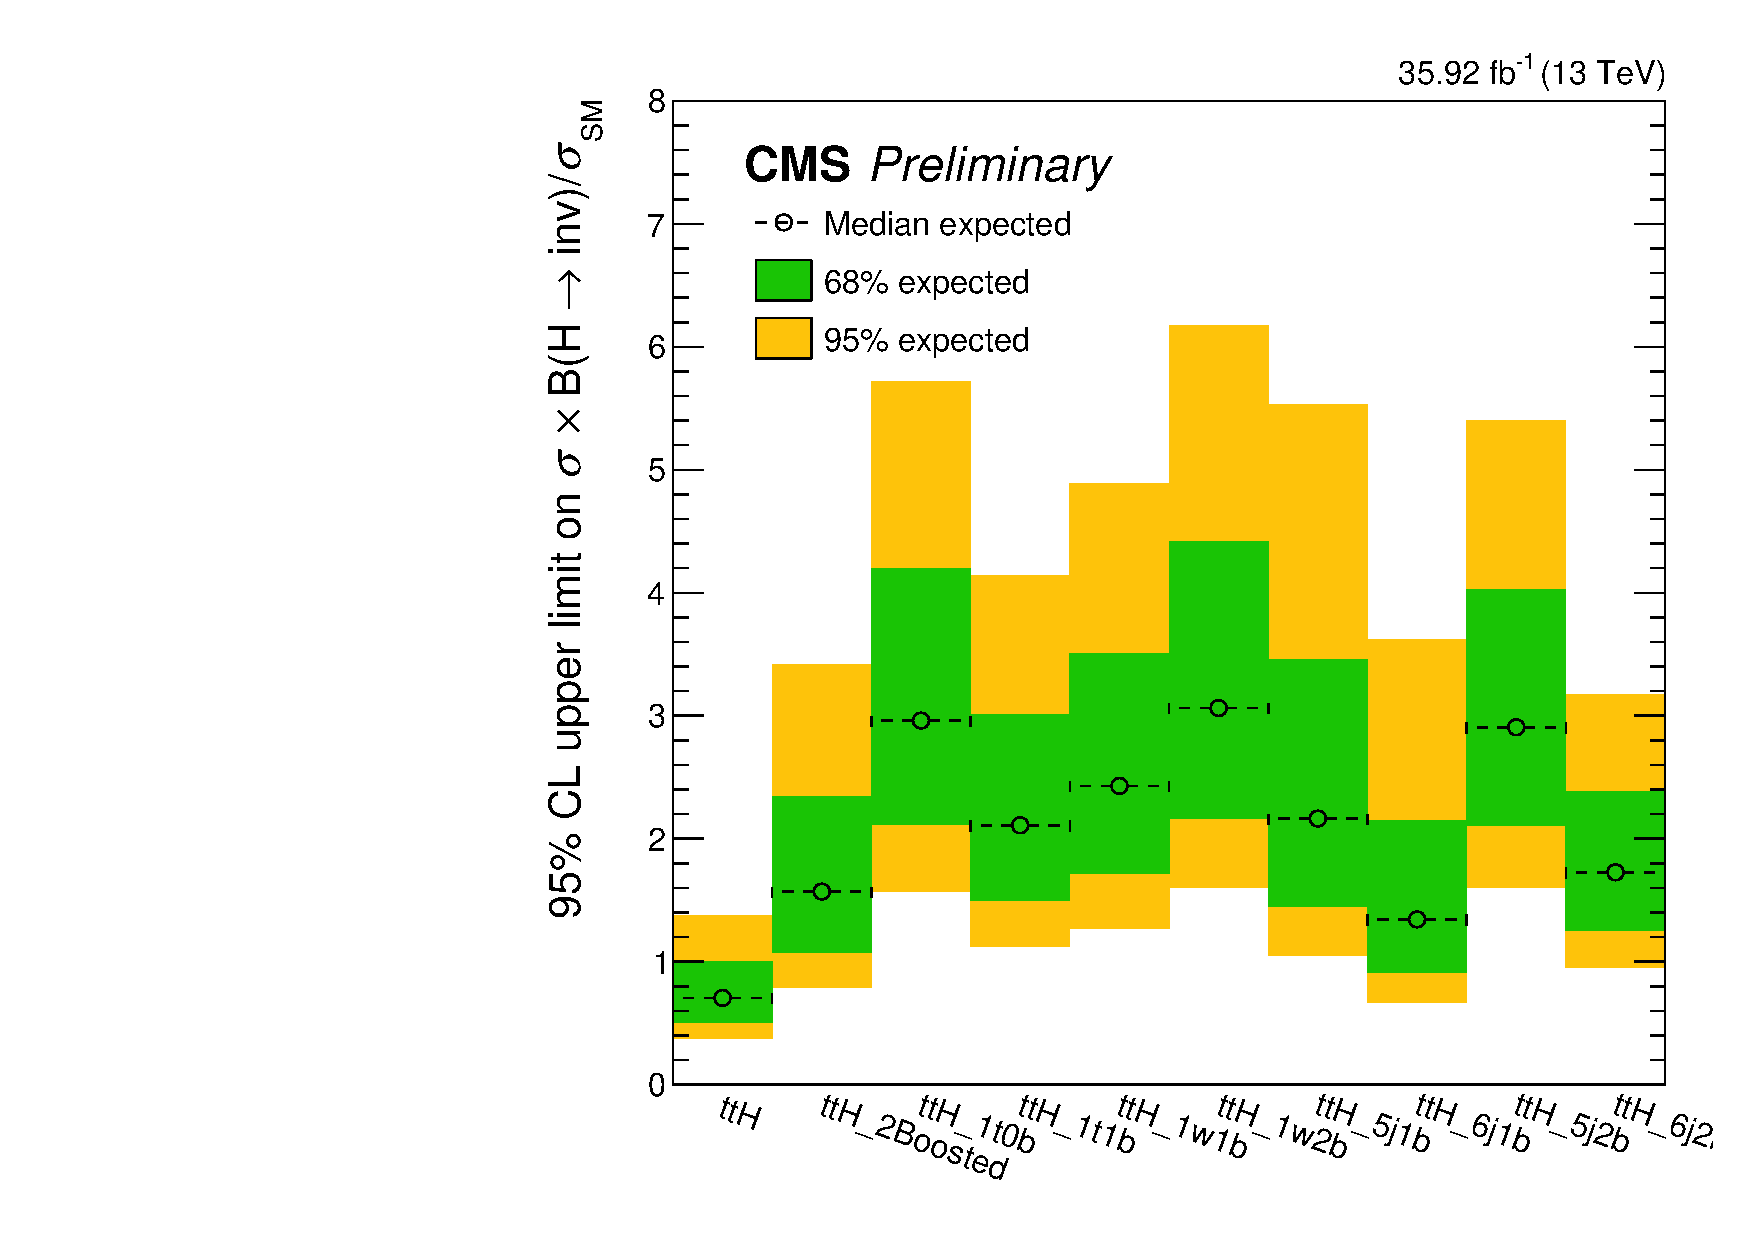
\includegraphics[width=\textwidth]{figures/limits/ttH/limit_2016_ttH_Scenario5.pdf}
        \caption{\ttH --- 2016}
    \end{subfigure}
    \hfill
    \begin{subfigure}[b]{0.45\textwidth}
        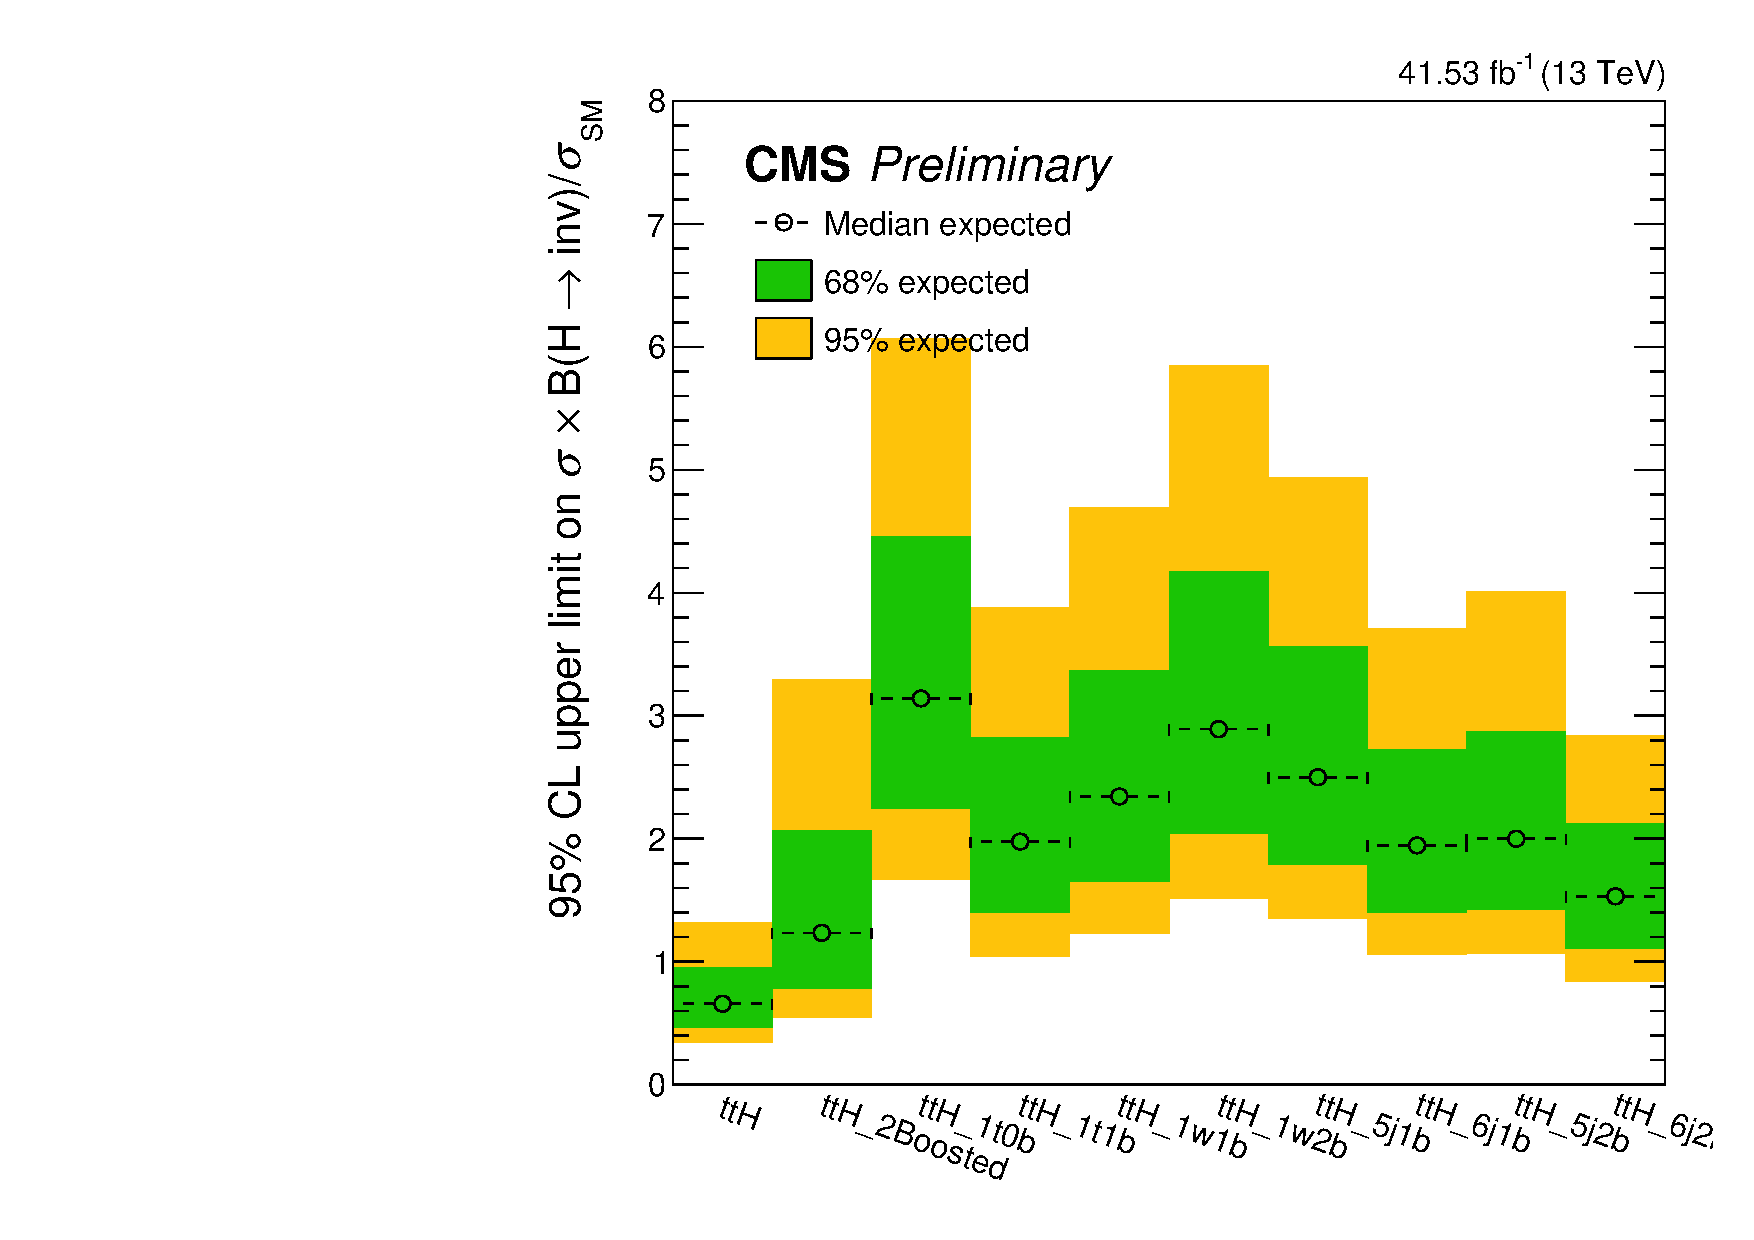
\includegraphics[width=\textwidth]{figures/limits/ttH/limit_2017_ttH_Scenario5.pdf}
        \caption{\ttH --- 2017}
    \end{subfigure}

    \begin{subfigure}[b]{0.45\textwidth}
        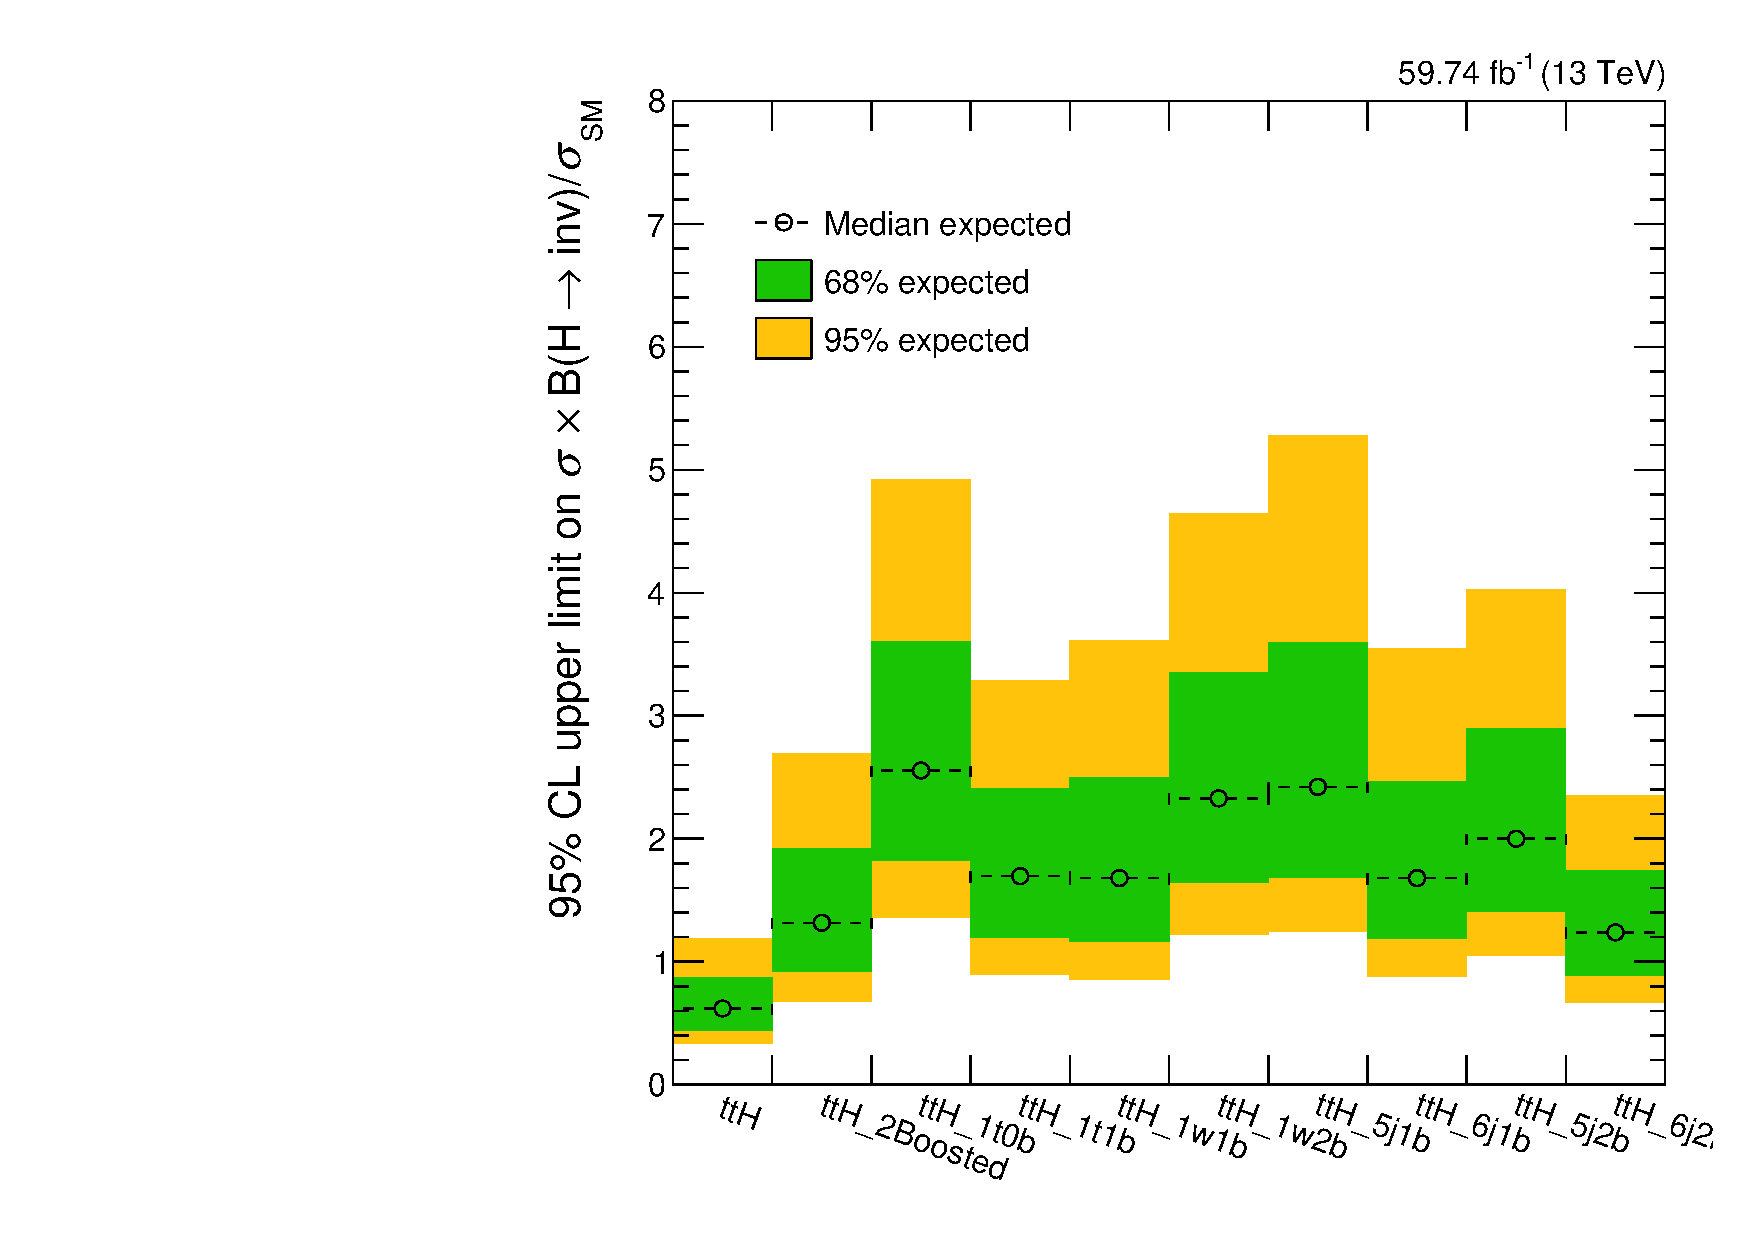
\includegraphics[width=\textwidth]{figures/limits/ttH/limit_2018_ttH_Scenario5.pdf}
        \caption{\ttH --- 2018}
    \end{subfigure}
    \hfill
    \begin{subfigure}[b]{0.45\textwidth}
        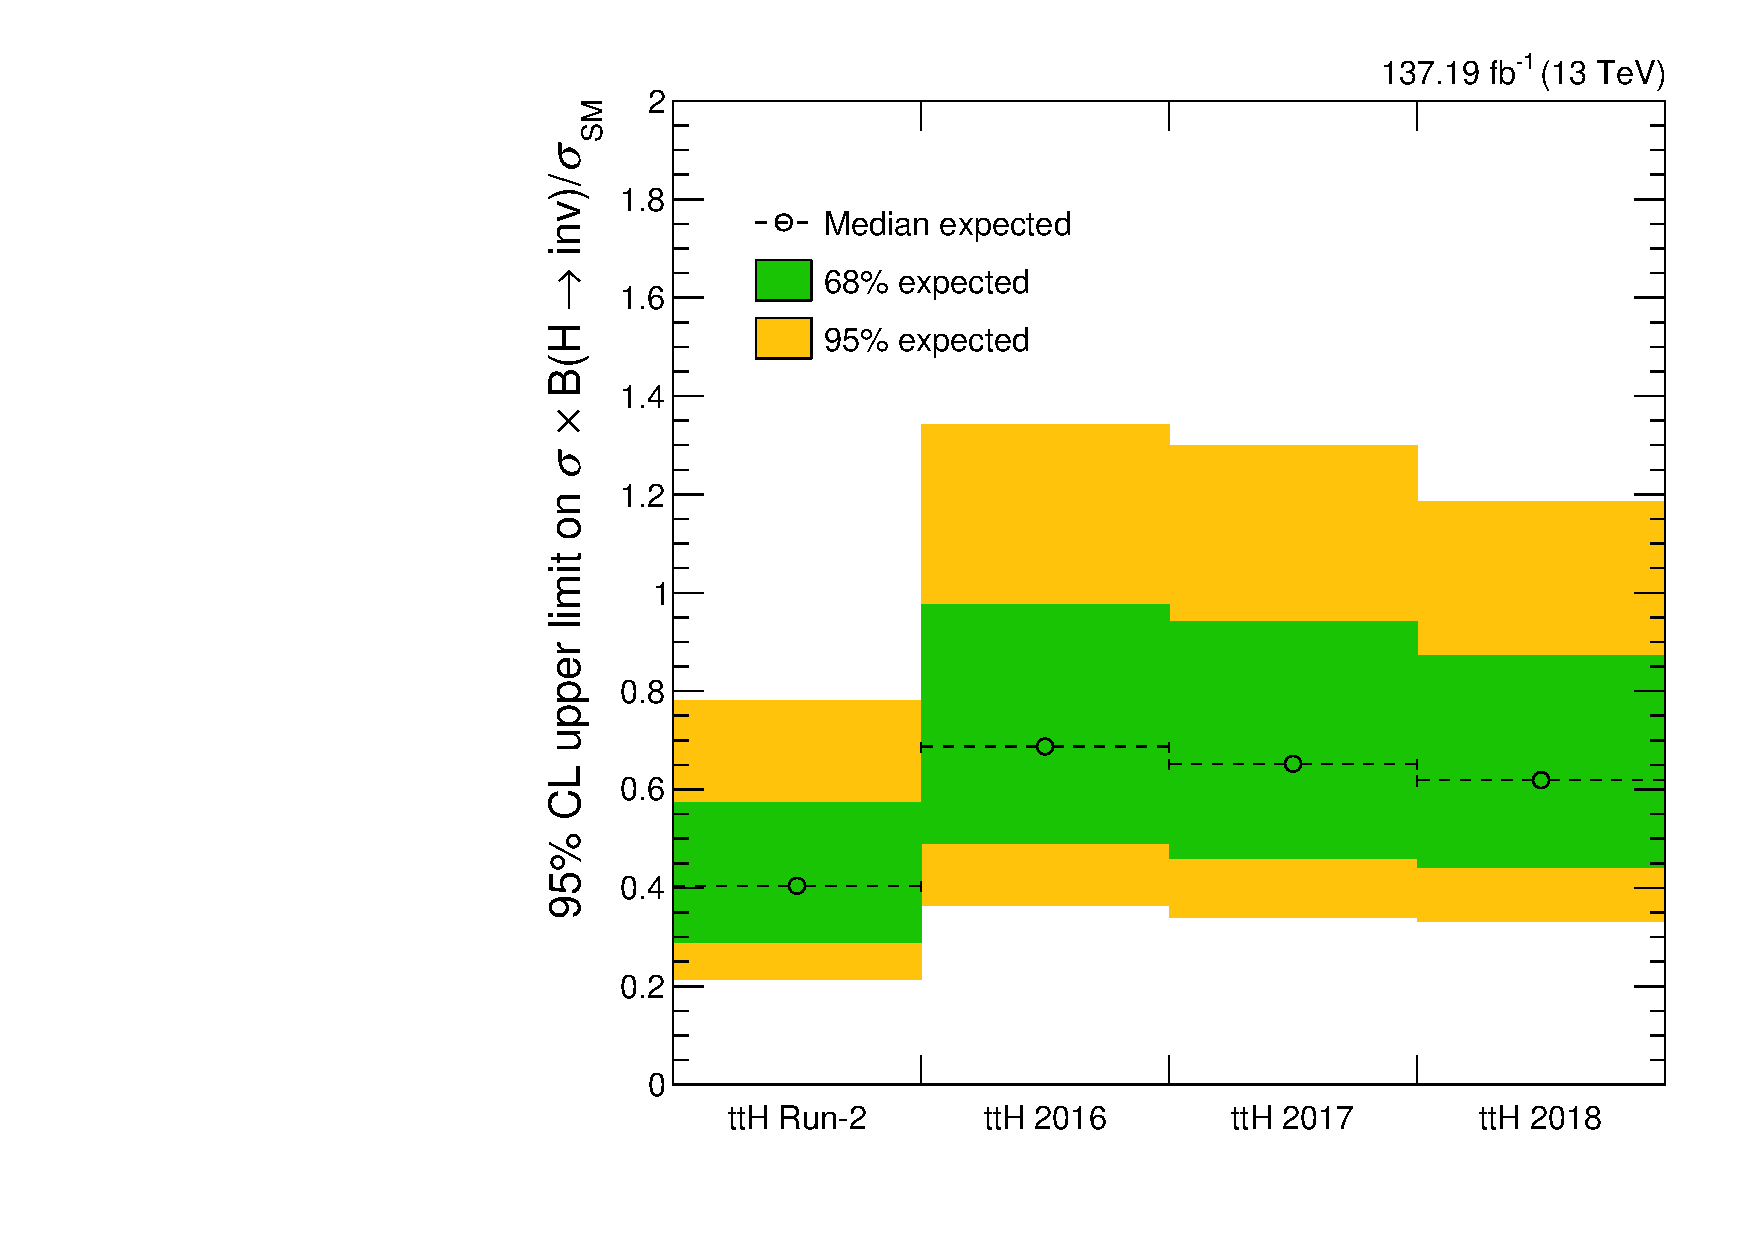
\includegraphics[width=\textwidth]{figures/limits/ttH/limit_Run2_ttH_Scenario5.pdf}
        \caption{\ttH --- Run-2}
    \end{subfigure}
    \caption[Expected 95\,\% CL upper limits on the Higgs boson to invisible state branching fraction in the \ttH category, for both the individual subcategories, and the combination of them, for each data-taking year in Run-2]{Expected 95\,\% CL upper limits on the Higgs boson to invisible state branching fraction in the \ttH category, for both the individual subcategories, and the combination of them, for each data-taking year in Run-2.}
    \label{fig:htoinv_limit_ttH}
\end{figure}


%=========================================================


\section{Analysis of the \texorpdfstring{\VH}{VH} mode}
\label{sec:htoinv_analysis_VH}

% Describe the specifics of the background estimation and fit for the VH subcategories, since they may differ for the other modes

Fig.~\ref{fig:htoinv_limit_VH} showcases the median expected limit on $\BRof{\higgstoinv}$ with 1$\sigma$ and 2$\sigma$ bounds for the \VH category and its subcategories.

\begin{figure}[htbp]
    \centering
    \begin{subfigure}[b]{0.45\textwidth}
        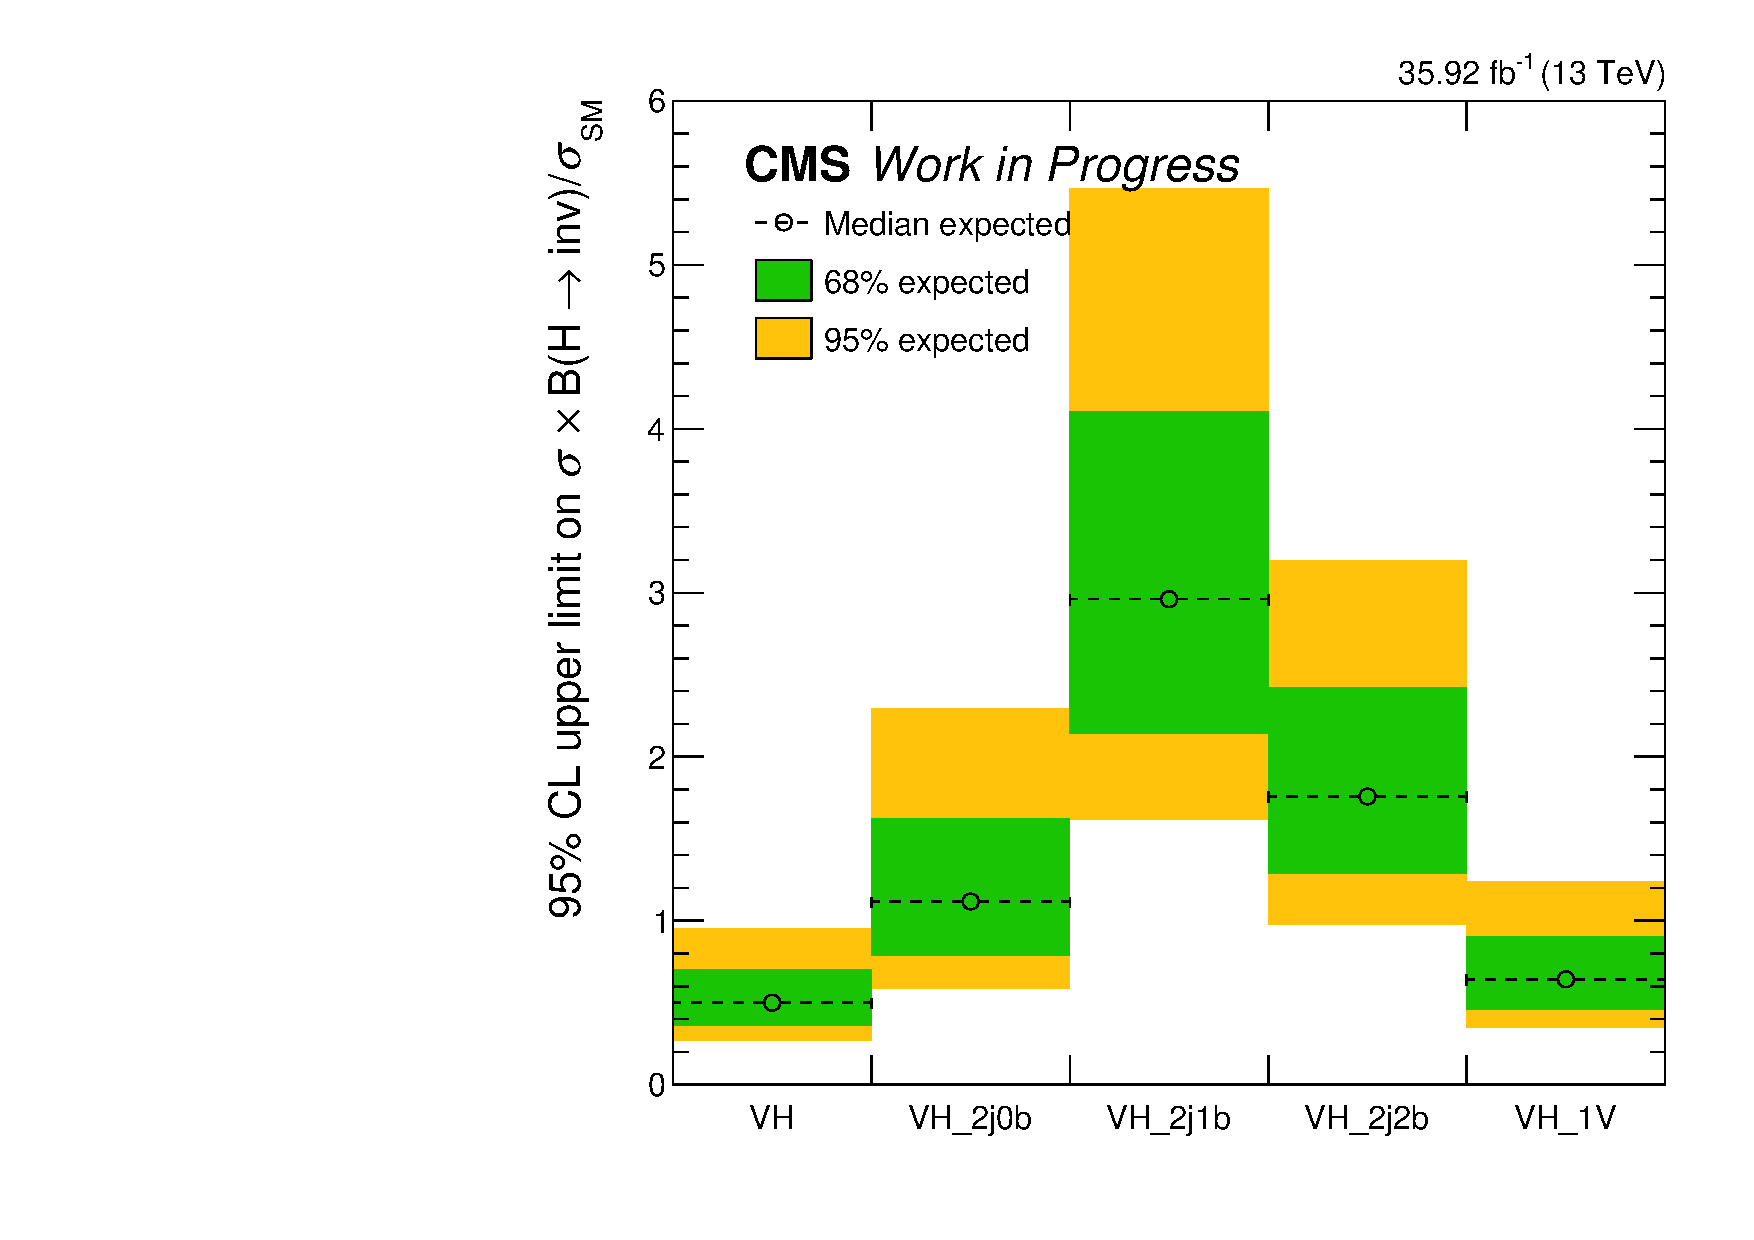
\includegraphics[width=\textwidth]{figures/limits/VH/limit_2016_VH_Scenario5.pdf}
        \caption{\VH --- 2016}
    \end{subfigure}
    \hfill
    \begin{subfigure}[b]{0.45\textwidth}
        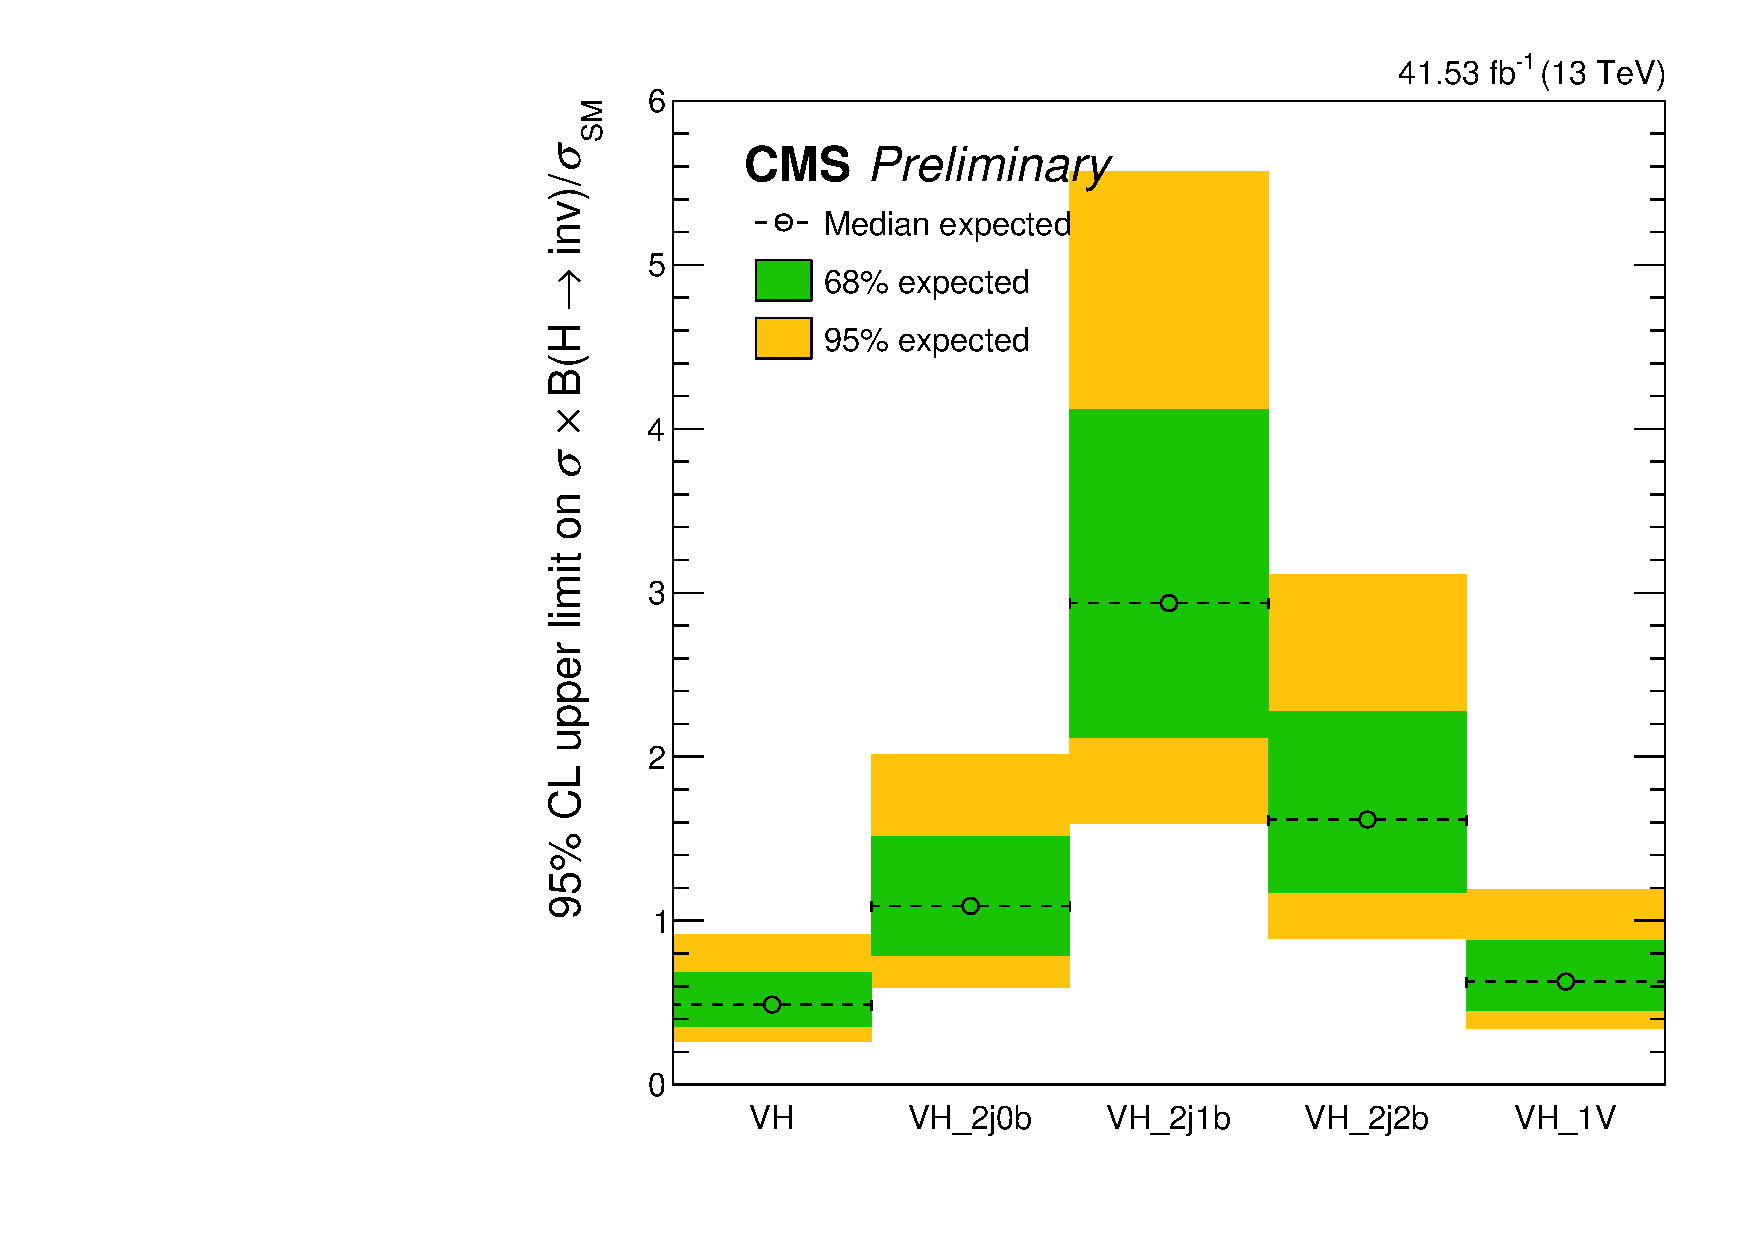
\includegraphics[width=\textwidth]{figures/limits/VH/limit_2017_VH_Scenario5.pdf}
        \caption{\VH --- 2017}
    \end{subfigure}

    \begin{subfigure}[b]{0.45\textwidth}
        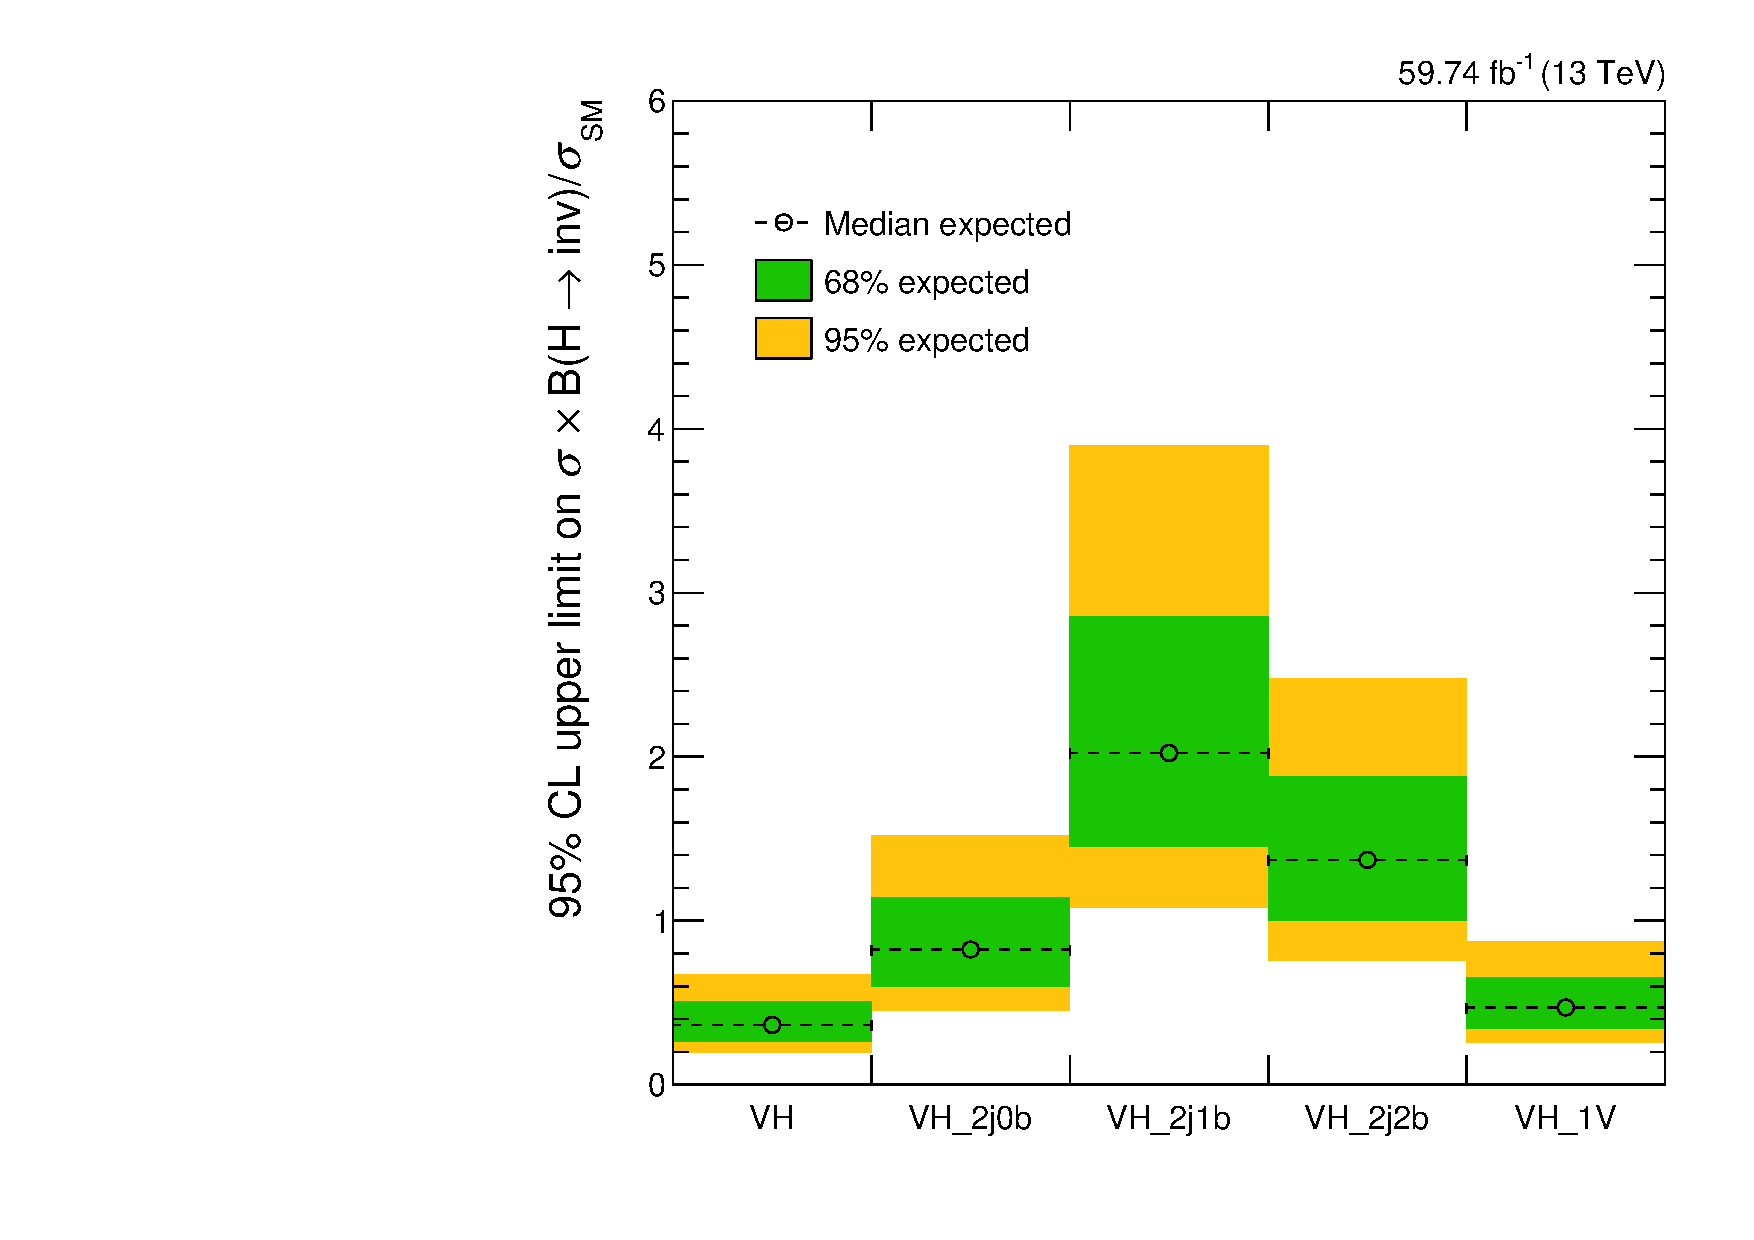
\includegraphics[width=\textwidth]{figures/limits/VH/limit_2018_VH_Scenario5.pdf}
        \caption{\VH --- 2018}
    \end{subfigure}
    \hfill
    \begin{subfigure}[b]{0.45\textwidth}
        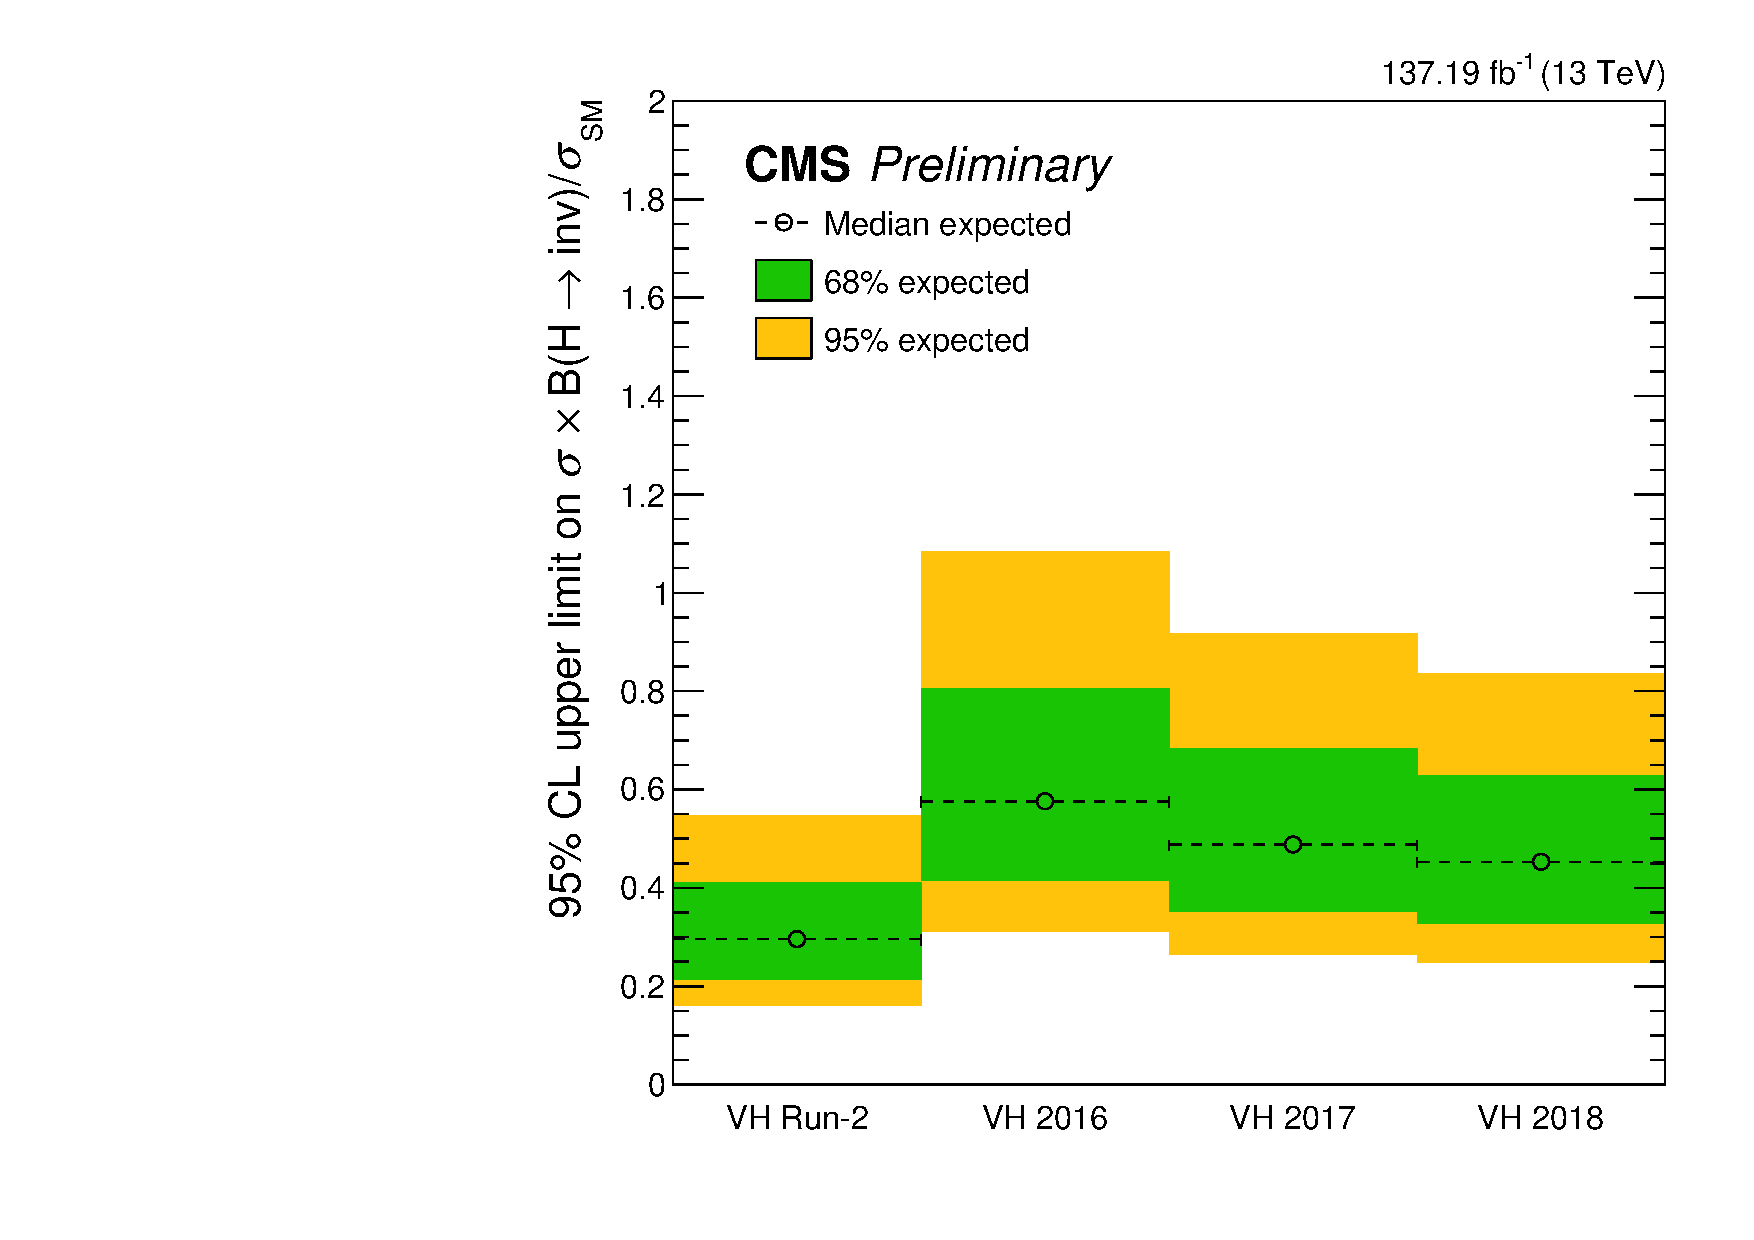
\includegraphics[width=\textwidth]{figures/limits/VH/limit_Run2_VH_Scenario5.pdf}
        \caption{\VH --- Run-2}
    \end{subfigure}
    \caption[Expected 95\,\% CL upper limits on the Higgs boson to invisible state branching fraction in the \VH category, for both the individual subcategories, and the combination of them, for each data-taking year in Run-2]{Expected 95\,\% CL upper limits on the Higgs boson to invisible state branching fraction in the \VH category, for both the individual subcategories, and the combination of them, for each data-taking year in Run-2.}
    \label{fig:htoinv_limit_VH}
\end{figure}


%=========================================================


\section{Analysis of the \texorpdfstring{\ggH}{ggH} mode}
\label{sec:htoinv_analysis_ggF}

% Describe the specifics of the background estimation and fit for ggF subcategories, since they may differ for the other modes

Fig.~\ref{fig:htoinv_limit_ggF} showcases the median expected limit on $\BRof{\higgstoinv}$ with 1$\sigma$ and 2$\sigma$ bounds for the \ggH category and its subcategories.

\begin{figure}[htbp]
    \centering
    \begin{subfigure}[b]{0.45\textwidth}
        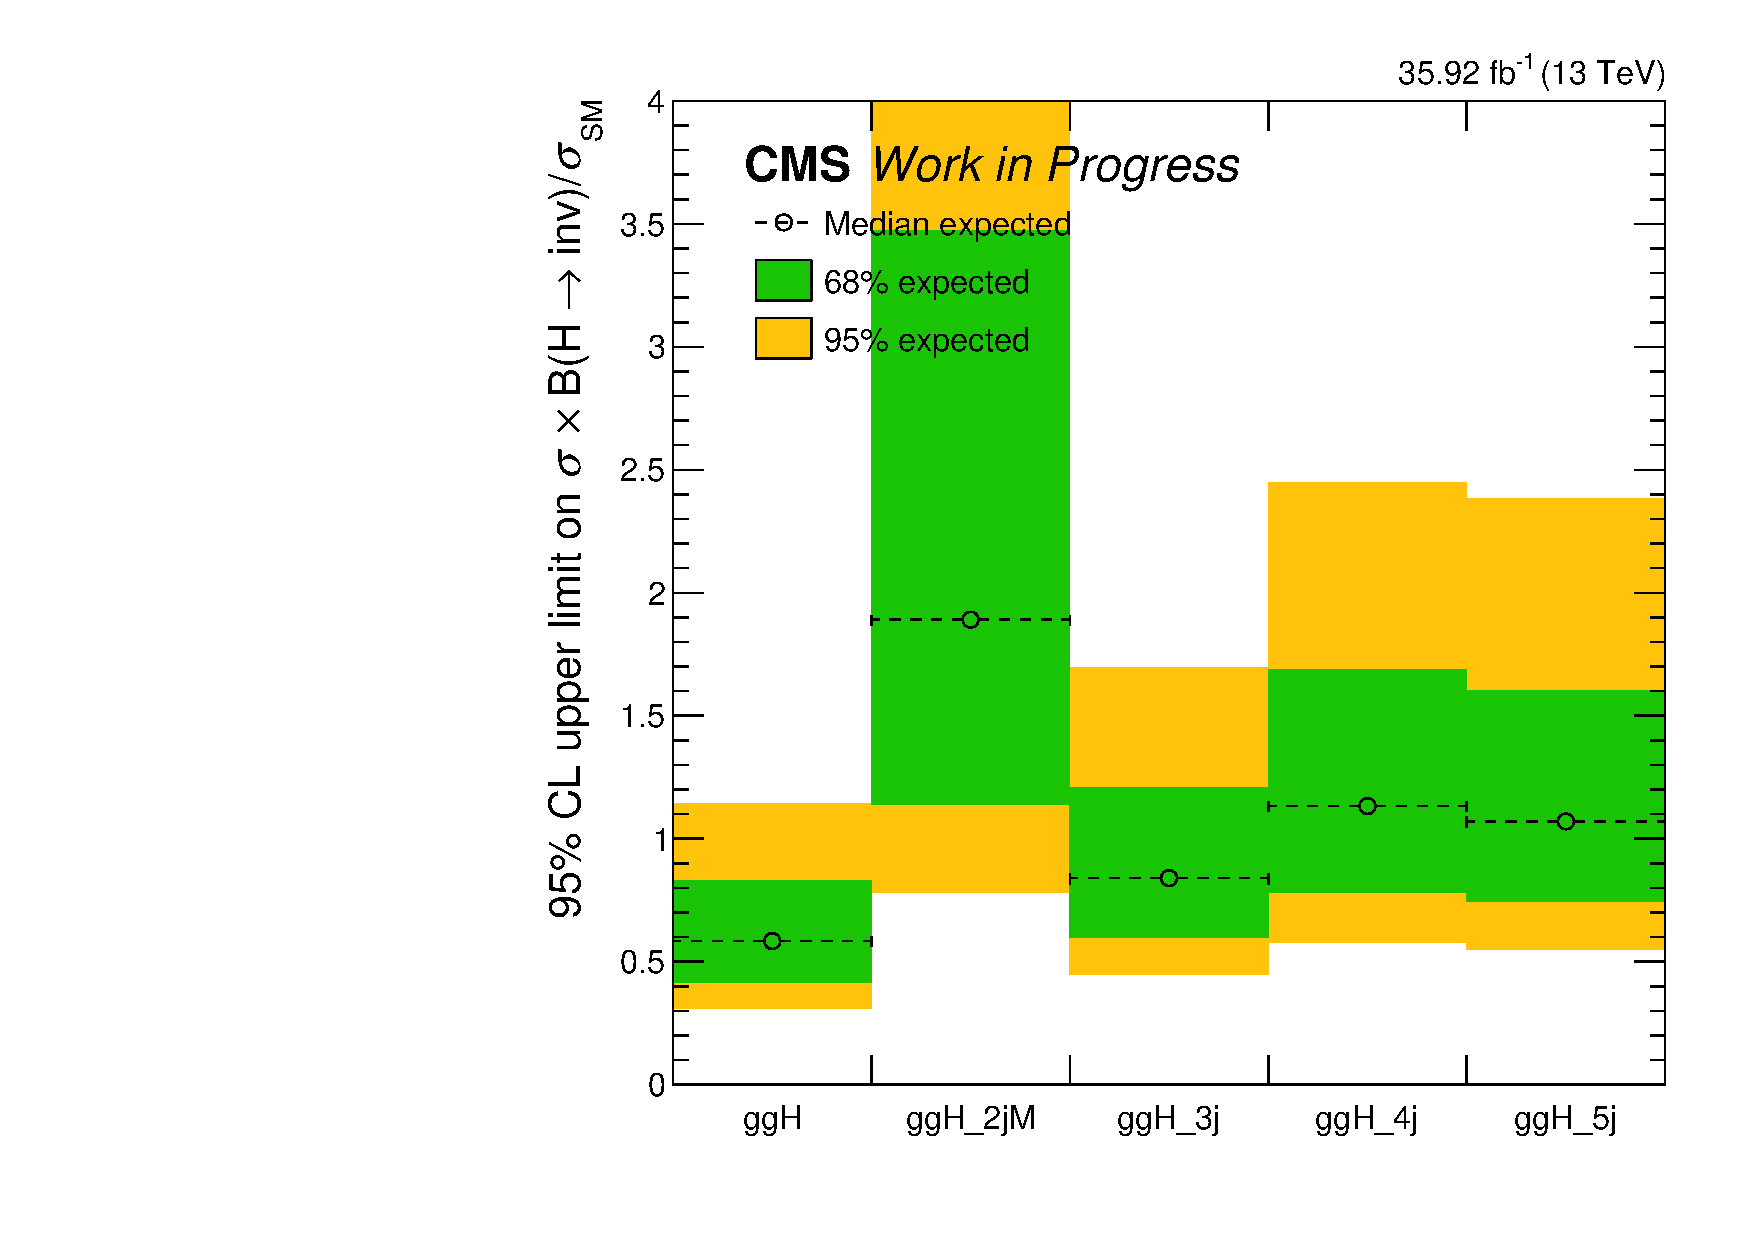
\includegraphics[width=\textwidth]{figures/limits/ggF/limit_2016_ggF_Scenario5.pdf}
        \caption{\ggH --- 2016}
    \end{subfigure}
    \hfill
    \begin{subfigure}[b]{0.45\textwidth}
        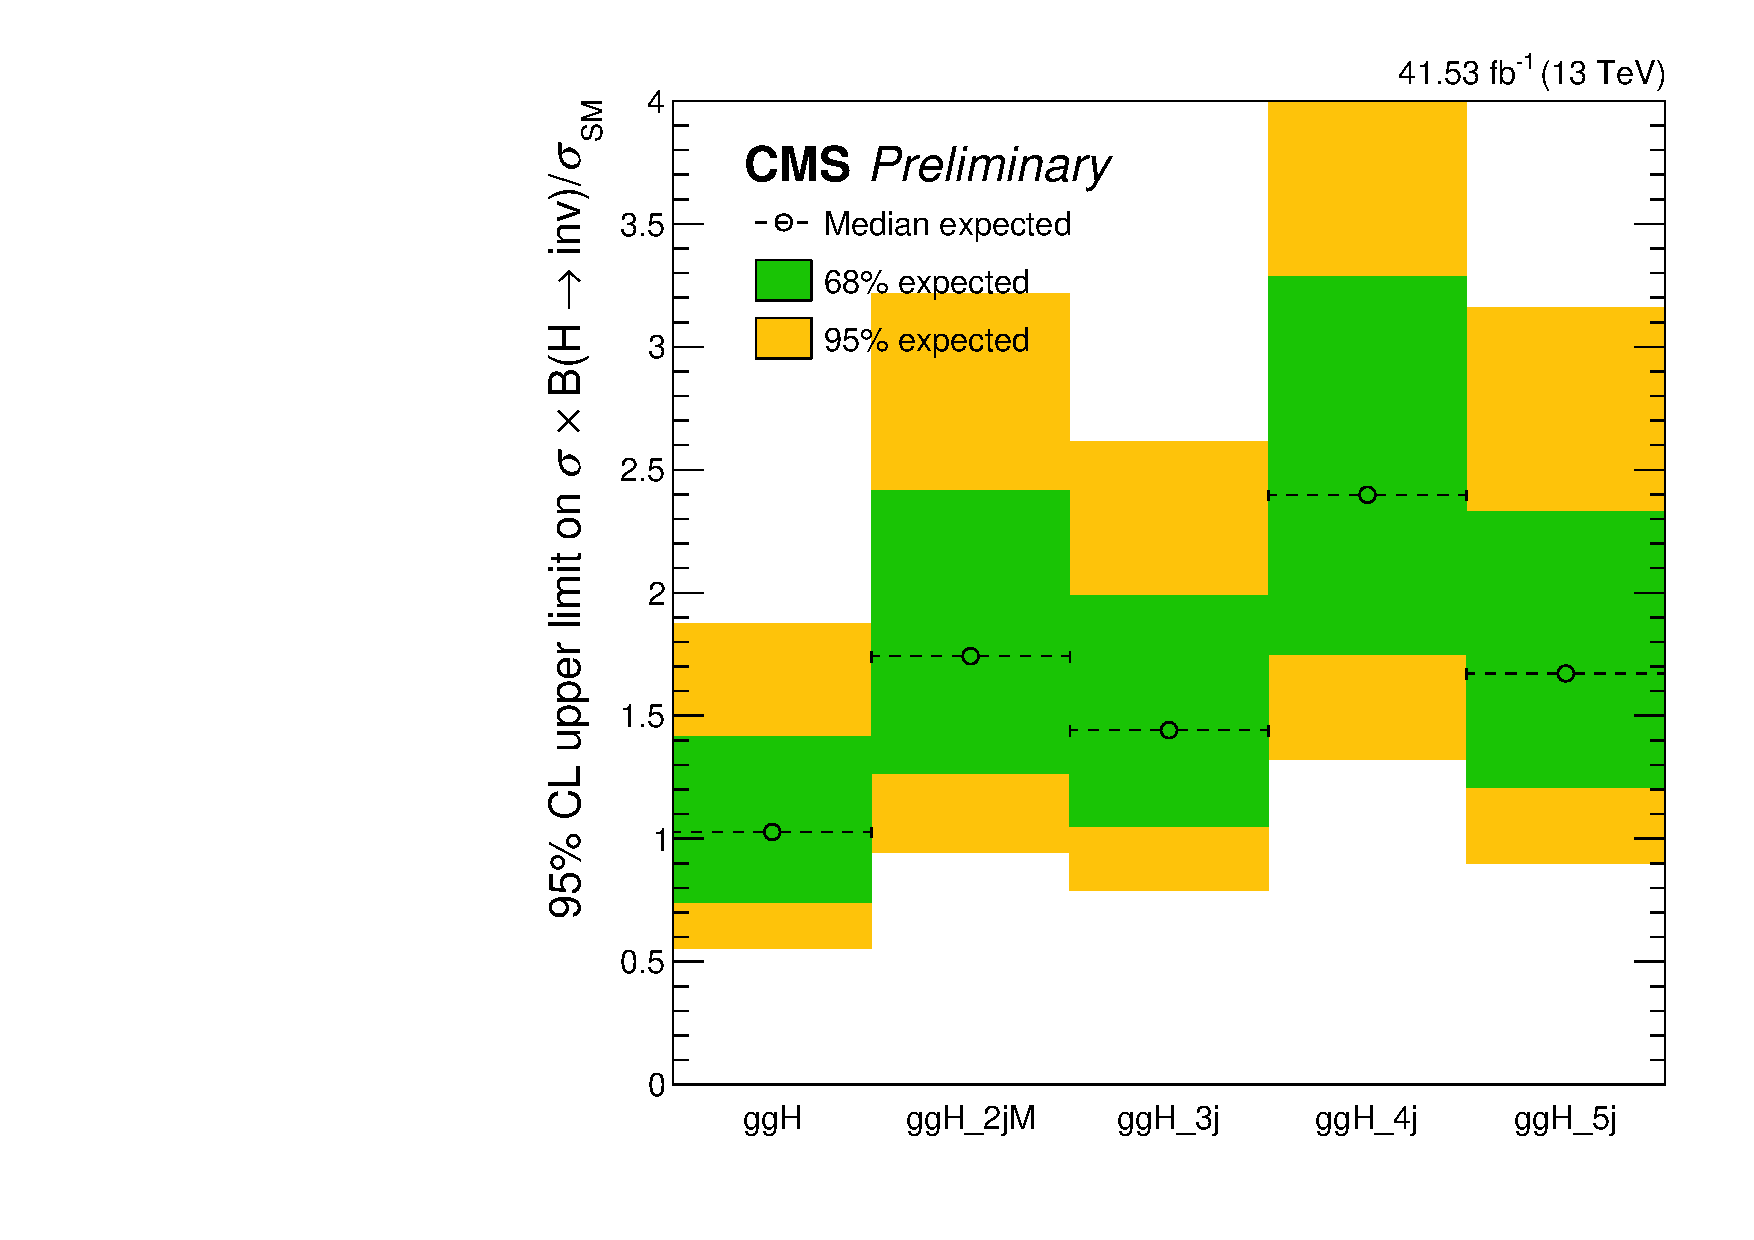
\includegraphics[width=\textwidth]{figures/limits/ggF/limit_2017_ggF_Scenario5.pdf}
        \caption{\ggH --- 2017}
    \end{subfigure}

    \begin{subfigure}[b]{0.45\textwidth}
        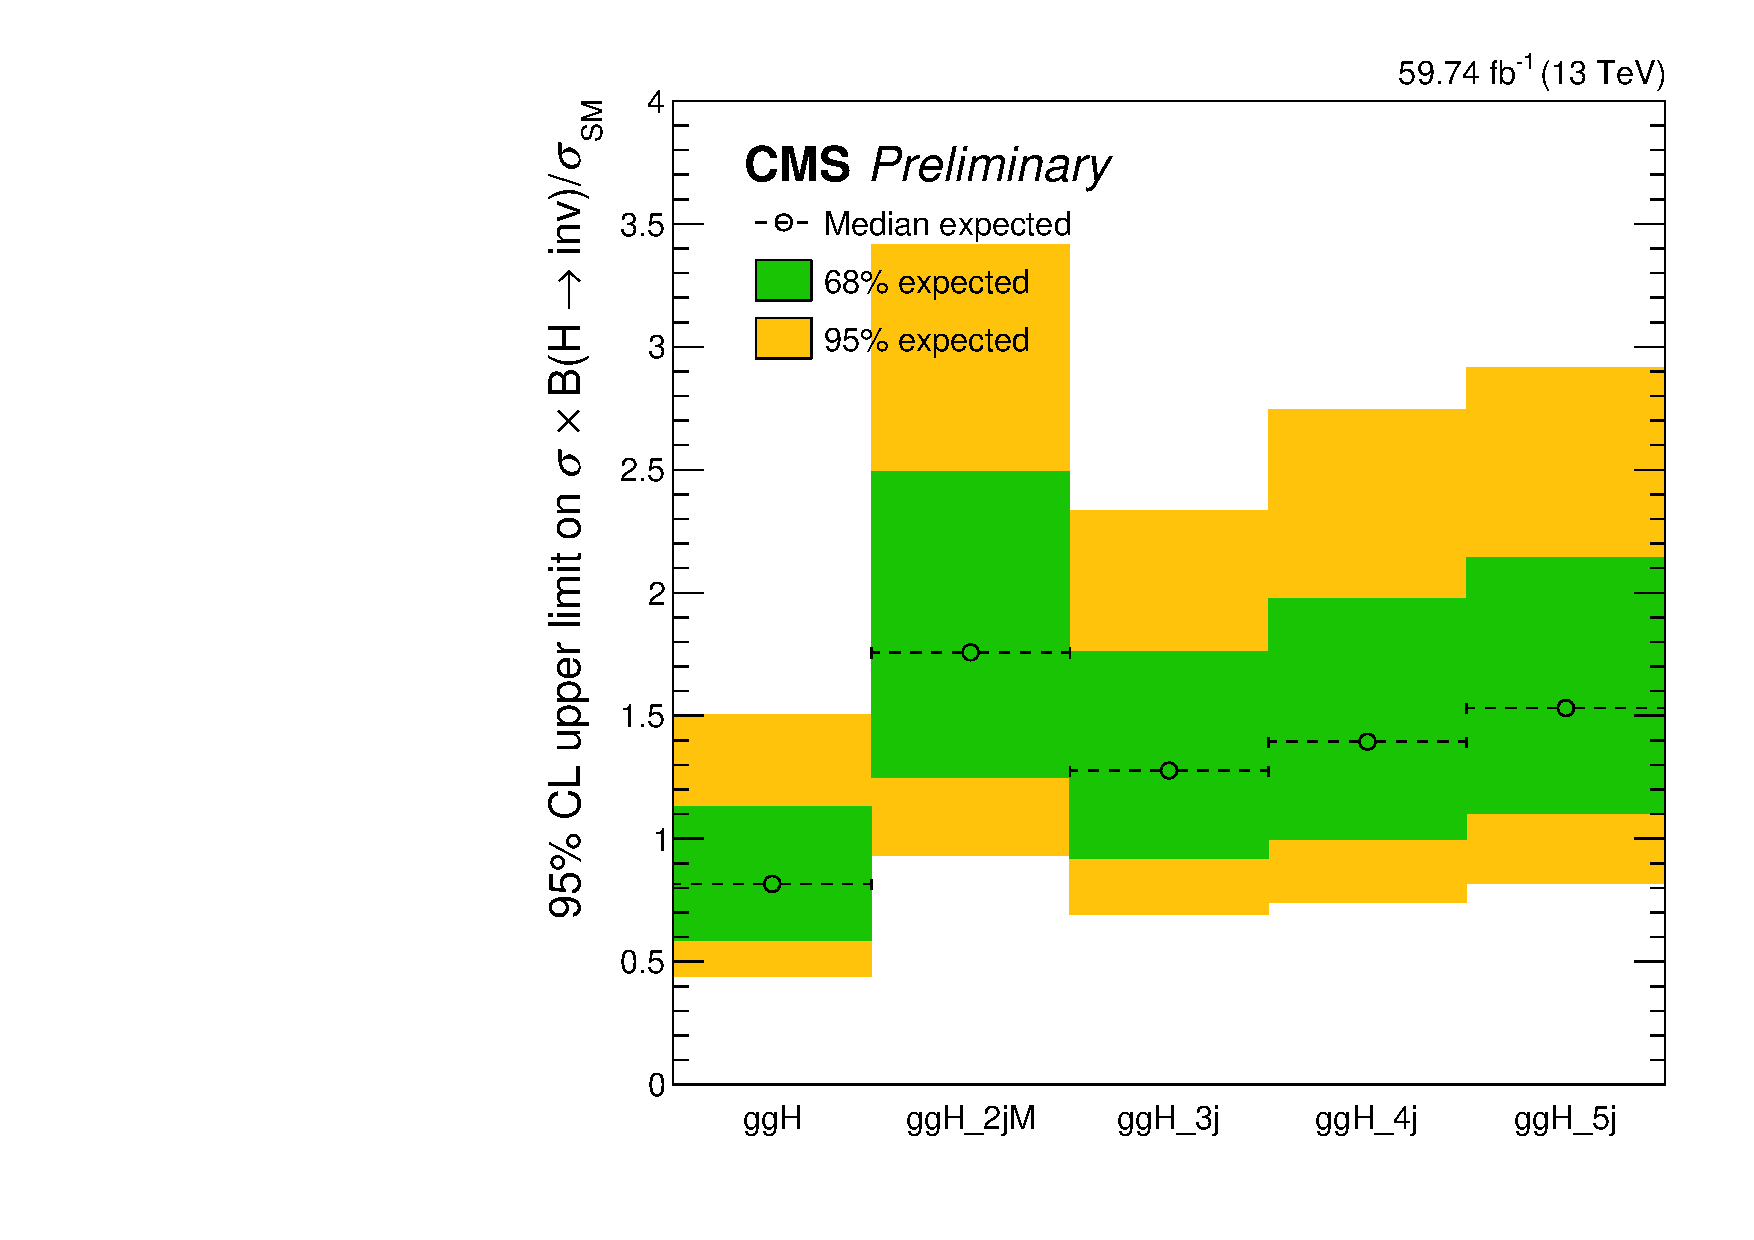
\includegraphics[width=\textwidth]{figures/limits/ggF/limit_2018_ggF_Scenario5.pdf}
        \caption{\ggH --- 2018}
    \end{subfigure}
    \hfill
    \begin{subfigure}[b]{0.45\textwidth}
        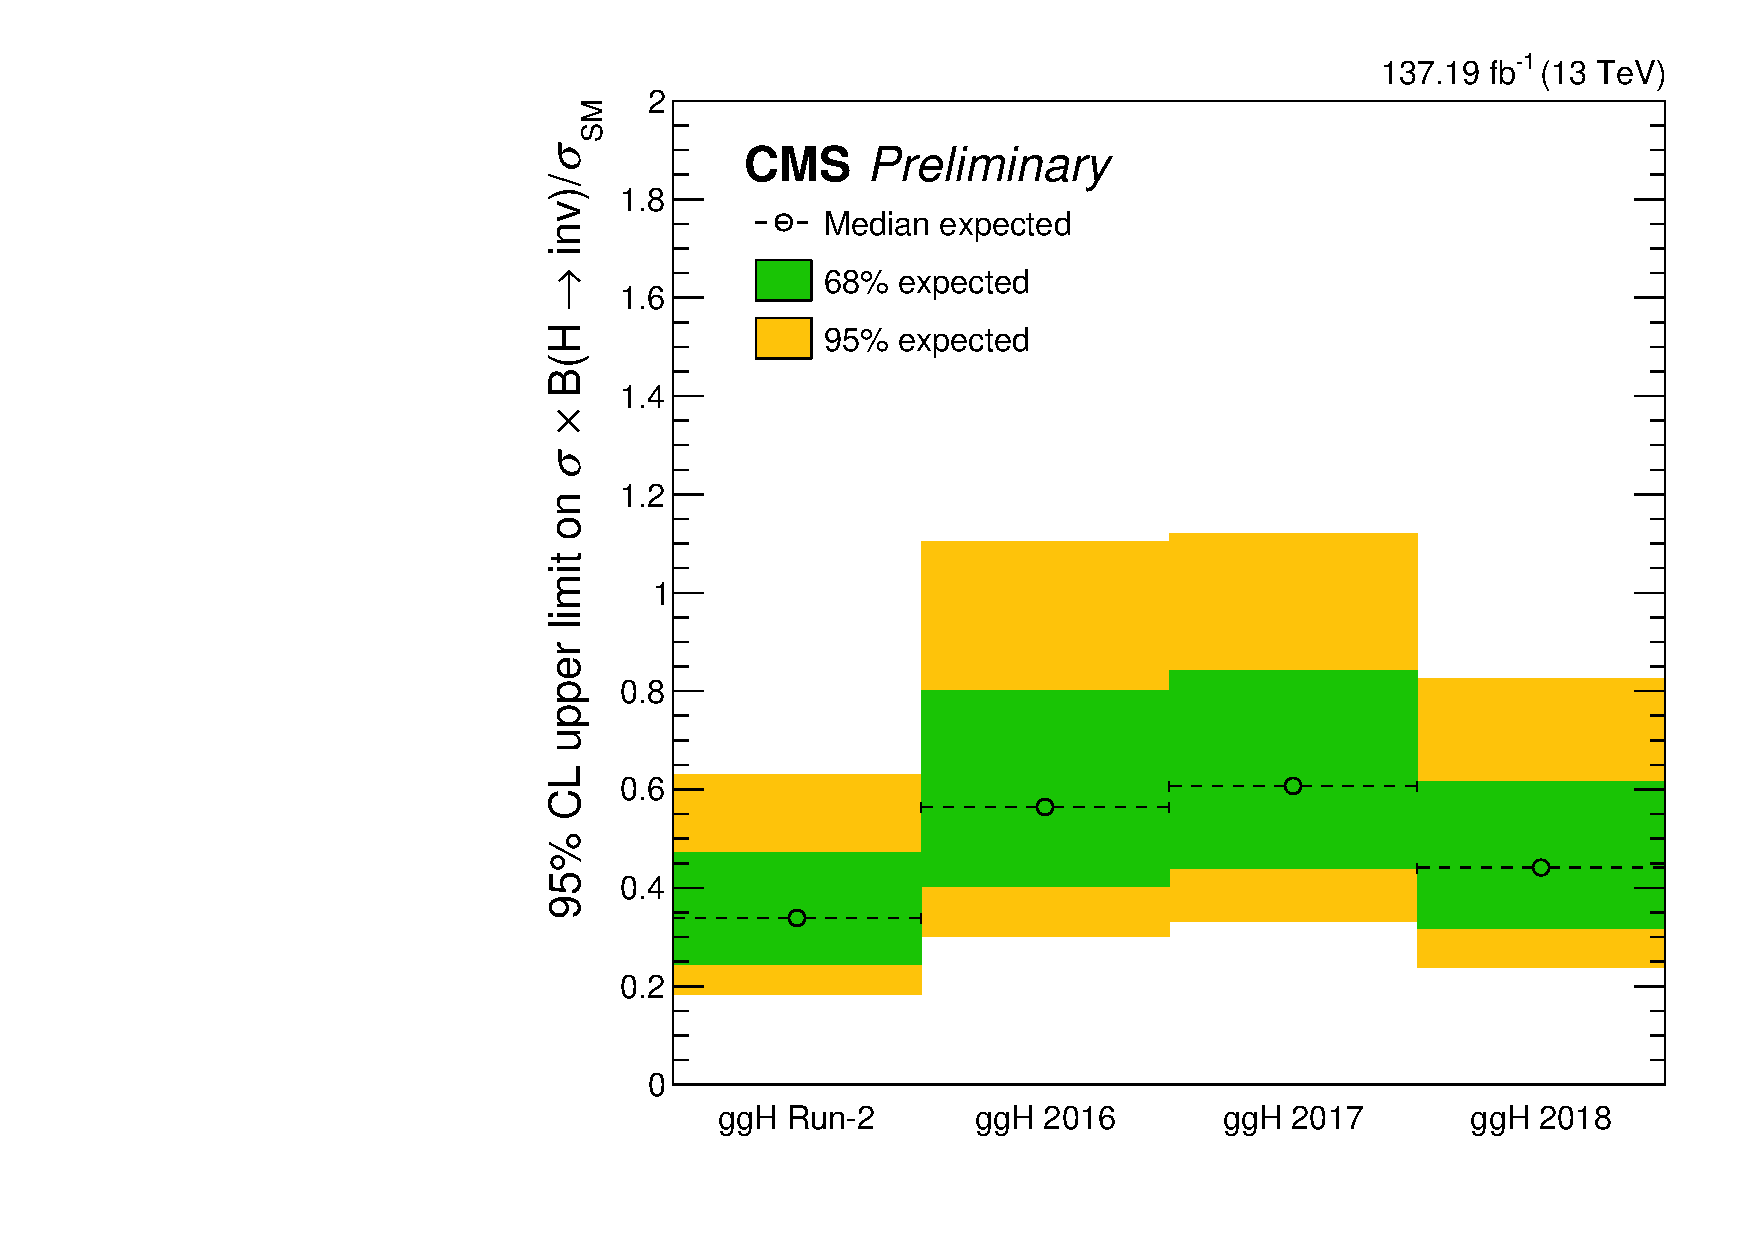
\includegraphics[width=\textwidth]{figures/limits/ggF/limit_Run2_ggF_Scenario5.pdf}
        \caption{\ggH --- Run-2}
    \end{subfigure}
    \caption[Expected 95\,\% CL upper limits on the Higgs boson to invisible state branching fraction in the \ggH category, for both the individual subcategories, and the combination of them, for each data-taking year in Run-2]{Expected 95\,\% CL upper limits on the Higgs boson to invisible state branching fraction in the \ggH category, for both the individual subcategories, and the combination of them, for each data-taking year in Run-2.}
    \label{fig:htoinv_limit_ggF}
\end{figure}


%=========================================================


\section{Combined results}
\label{sec:htoinv_combined_results}

% Show the results combined over all production modes (one plot for each year), then the full combination for Run-2, ideally with VBF results as well

Upper limits for $\BRof{\higgstoinv}$ by combining all categories for a given year are given for 2016, 2017, and 2018 in Figs.~\ref{fig:htoinv_limit_likelihood_2016}, \ref{fig:htoinv_limit_likelihood_2017}, \ref{fig:htoinv_limit_likelihood_2018}, respectively. For the full Run-2 dataset, they are broken down by data taking year in Fig.~\ref{fig:htoinv_limit_likelihood_Run2_per_year} and by category in Fig.~\ref{fig:htoinv_limit_likelihood_Run2_per_cat}.\footnote{Expected limits only, so far, and really only placeholders. The full Run-2 likelihood is not correct---fit fails to converge for most points.} Profile likelihood ratios as a function of $\BRof{\higgstoinv}$ are also presented opposite the limits.

\begin{figure}[htbp]
    \centering
    \begin{subfigure}[t]{0.45\textwidth}  % top align since figures are same dimensions, but x-axis labels are larger for likelihood
        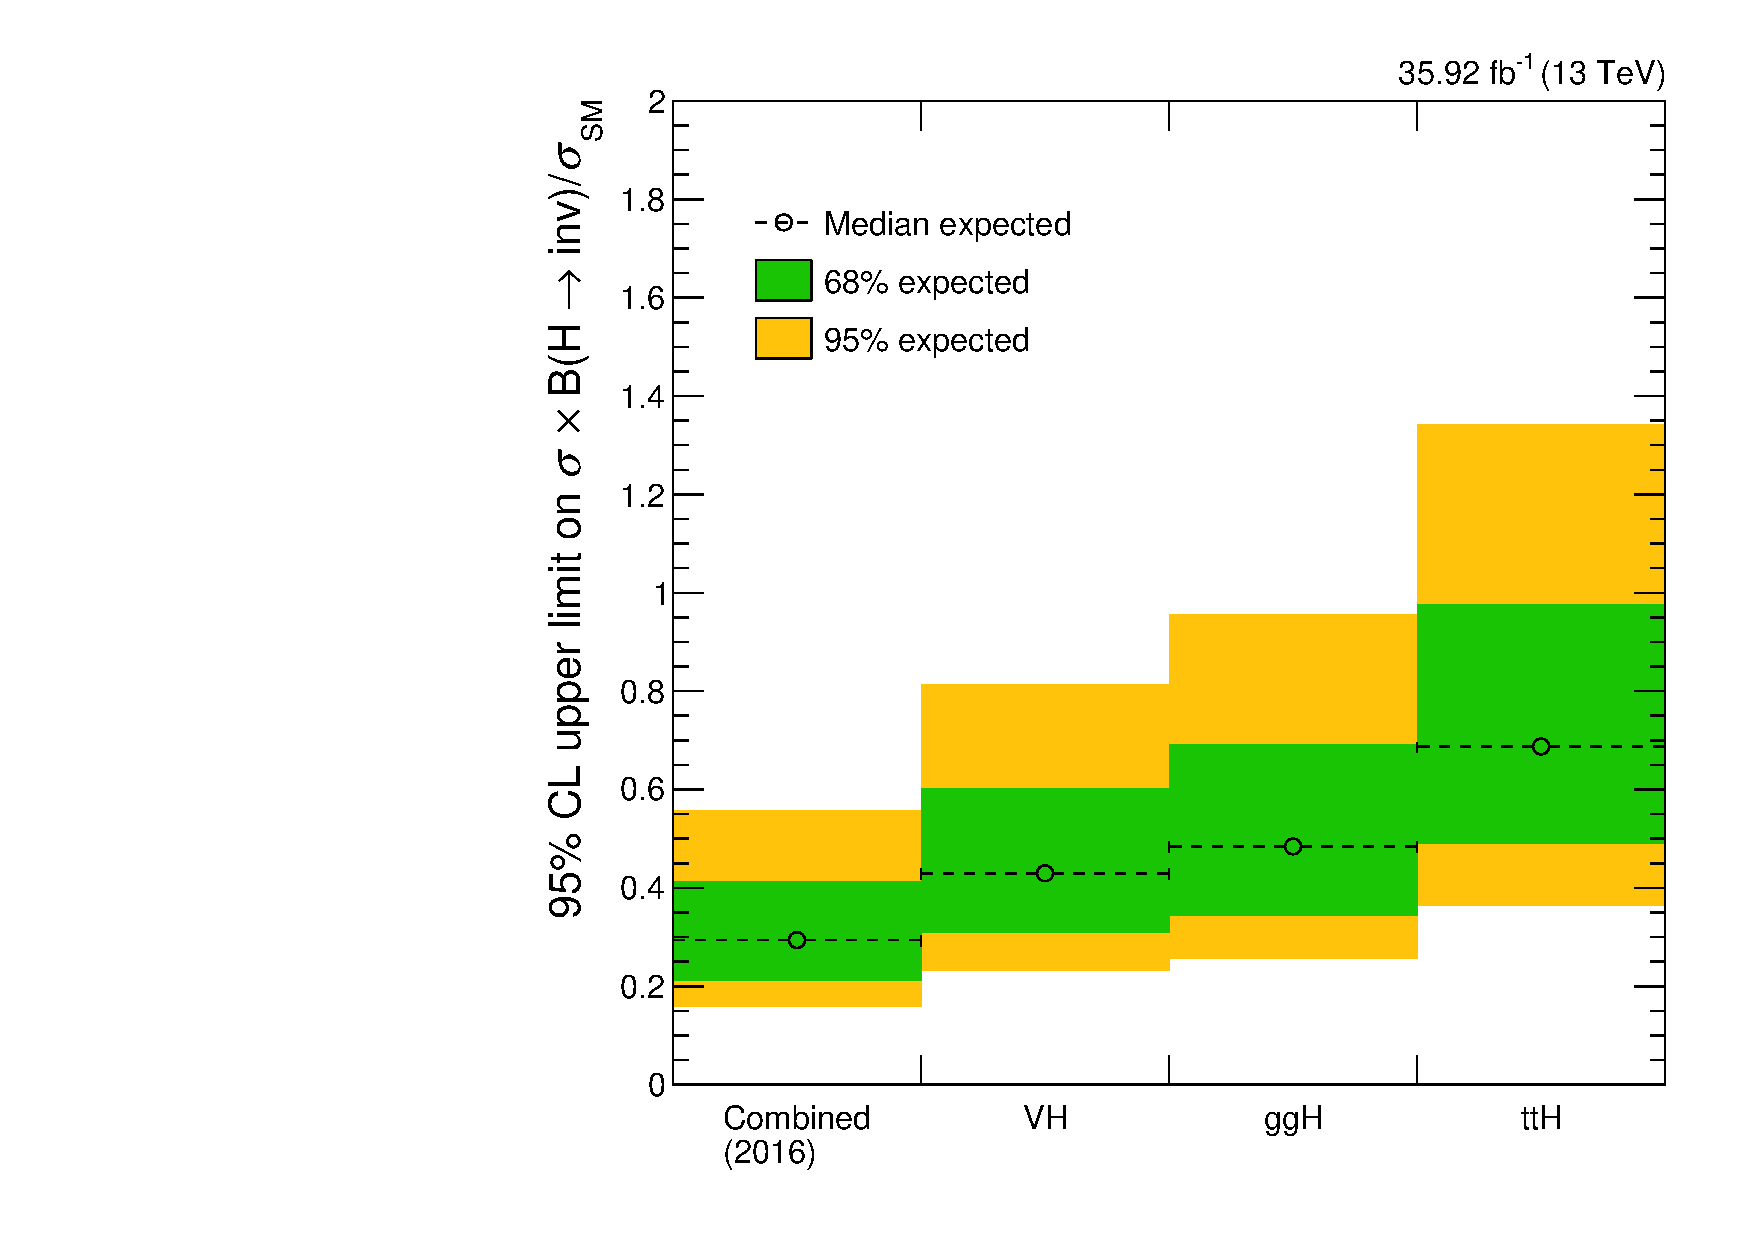
\includegraphics[width=\textwidth]{figures/limits/per_year/limit_2016_comb_Scenario5.pdf}
        \caption{Expected limit -- 2016}
    \end{subfigure}
    \hspace{0.05\textwidth}
    \begin{subfigure}[t]{0.45\textwidth}
        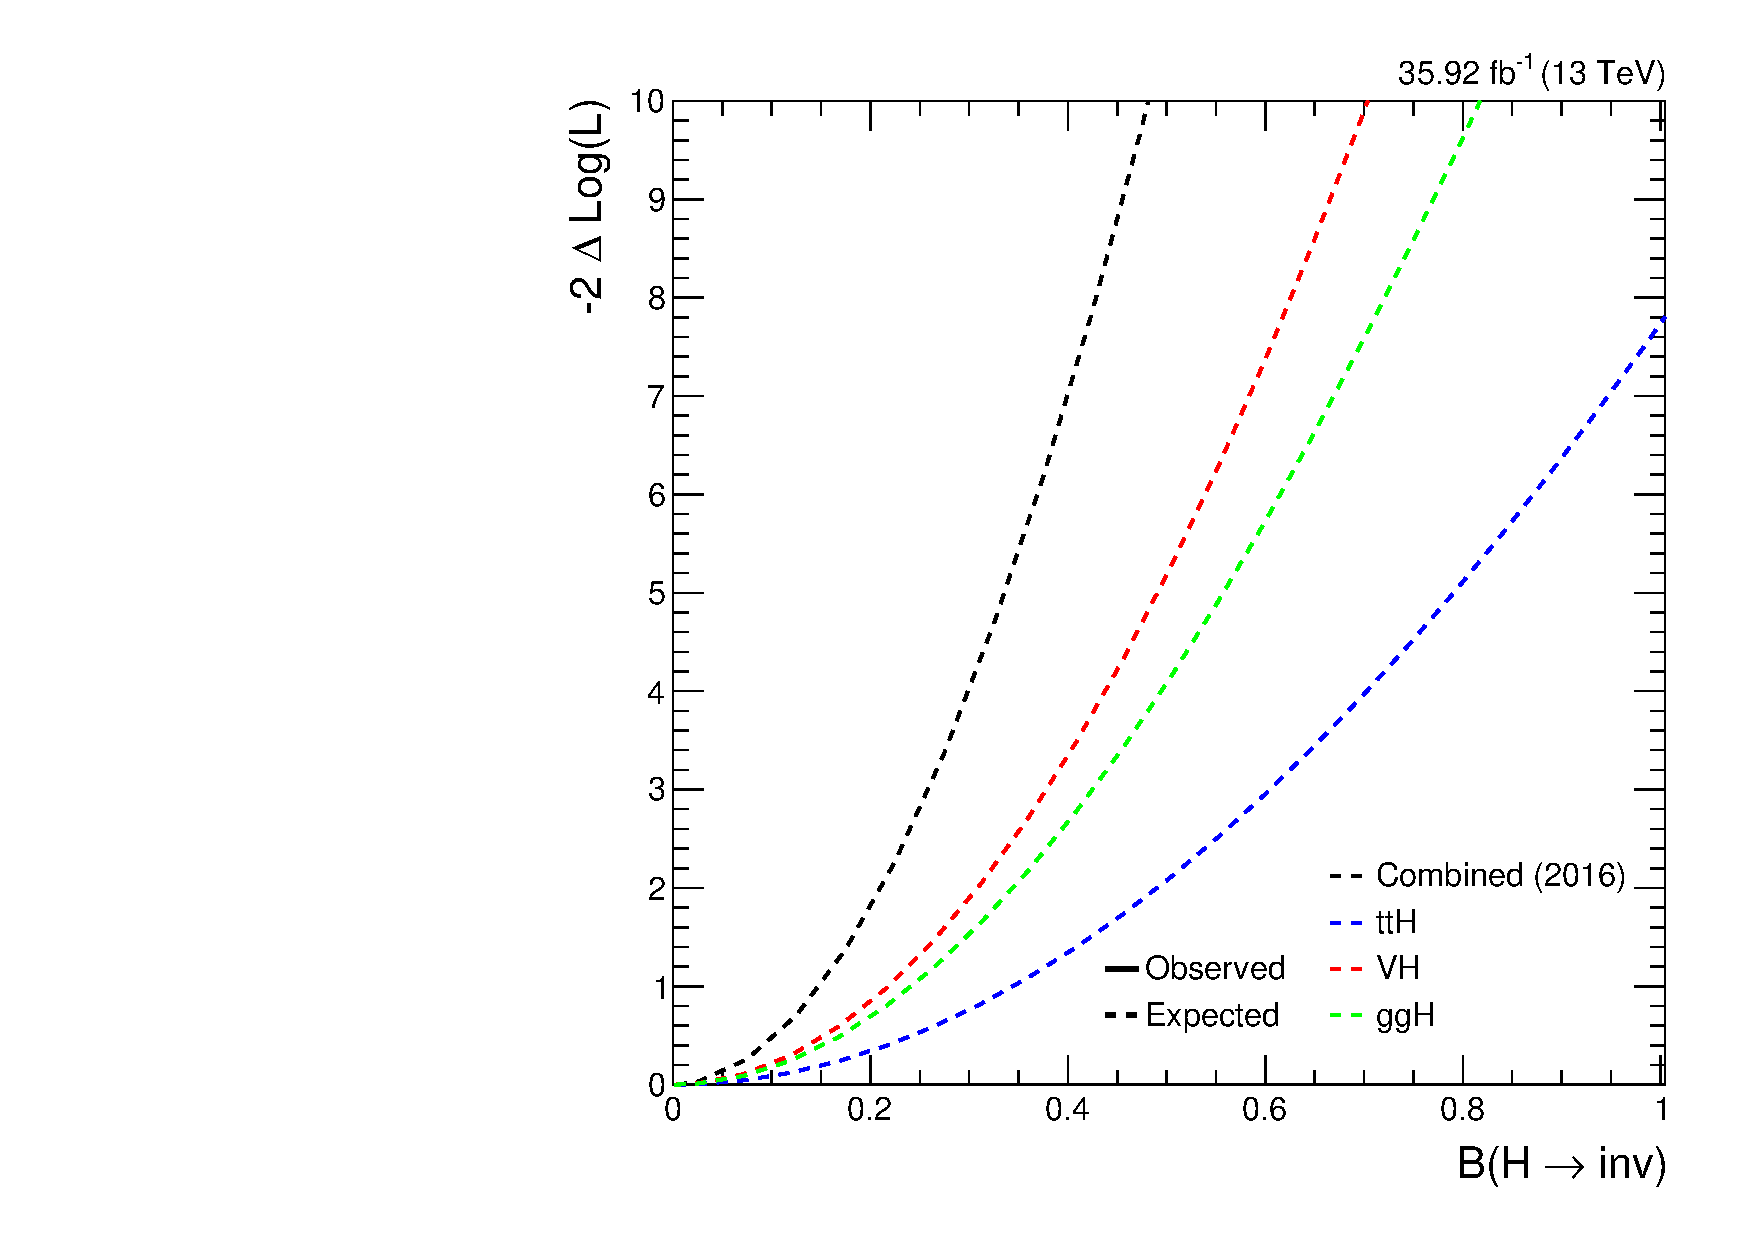
\includegraphics[width=\textwidth]{figures/likelihood_scan/profile_likelihood_scan_2016_Scenario5.pdf}
        \caption{Profile likelihood -- 2016}
    \end{subfigure}
    \caption[Expected 95\,\% CL upper limit on the Higgs boson to invisible state branching fraction $\BRof{\higgstoinv}$ and the corresponding profile likelihood ratio as a function of it, for both the individual categories that target a specific production mode, as well as the combination of them, for the 2016 dataset]{Expected 95\,\% CL upper limit on the Higgs boson to invisible state branching fraction $\BRof{\higgstoinv}$ (left) and the corresponding profile likelihood ratio as a function of it (right), for both the individual categories that target a specific production mode, as well as the combination of them, for the 2016 dataset. The \acrlong{sm} Higgs boson with its associated mass and production cross section are assumed.}
    \label{fig:htoinv_limit_likelihood_2016}
\end{figure}

\begin{figure}[htbp]
    \centering
    \begin{subfigure}[t]{0.45\textwidth}
        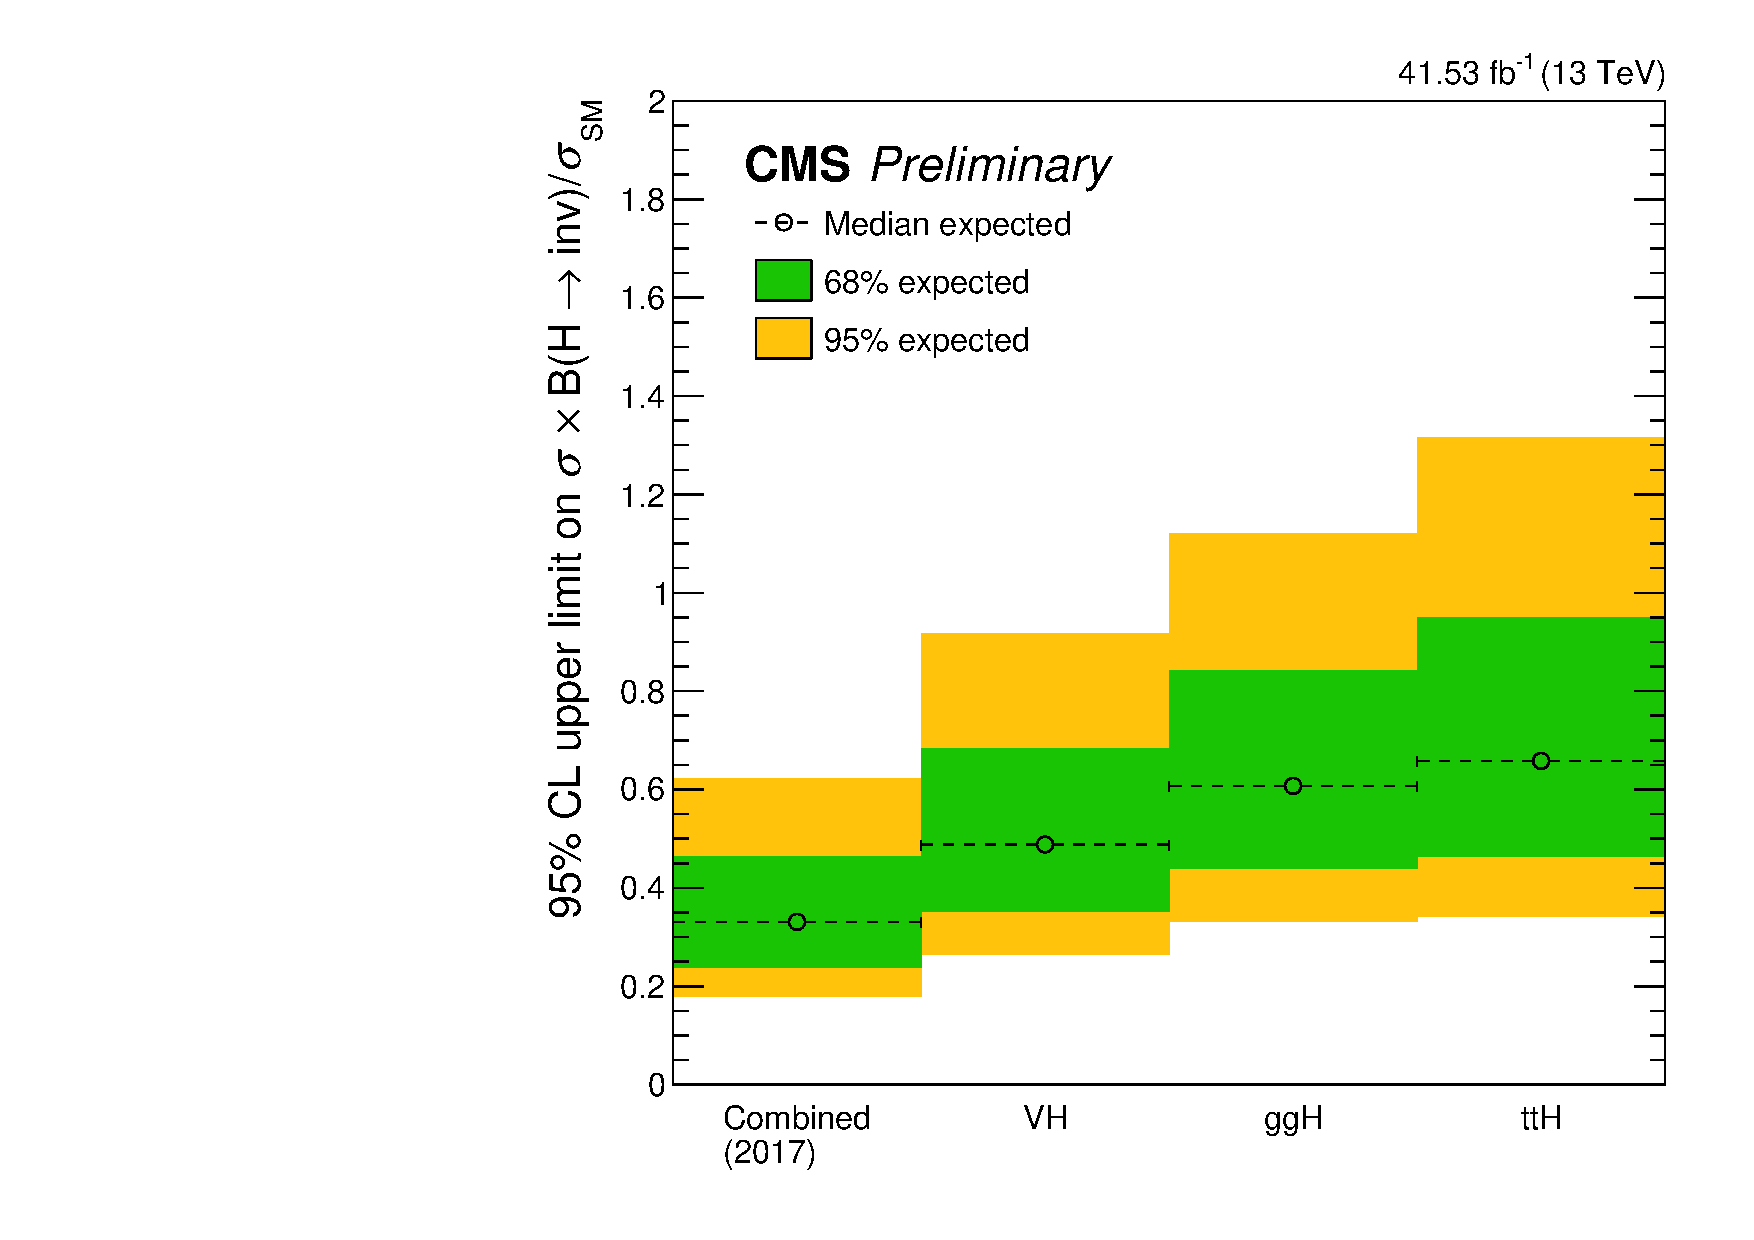
\includegraphics[width=\textwidth]{figures/limits/per_year/limit_2017_comb_Scenario5.pdf}
        \caption{Expected limit -- 2017}
    \end{subfigure}
    \hspace{0.05\textwidth}
    \begin{subfigure}[t]{0.45\textwidth}
        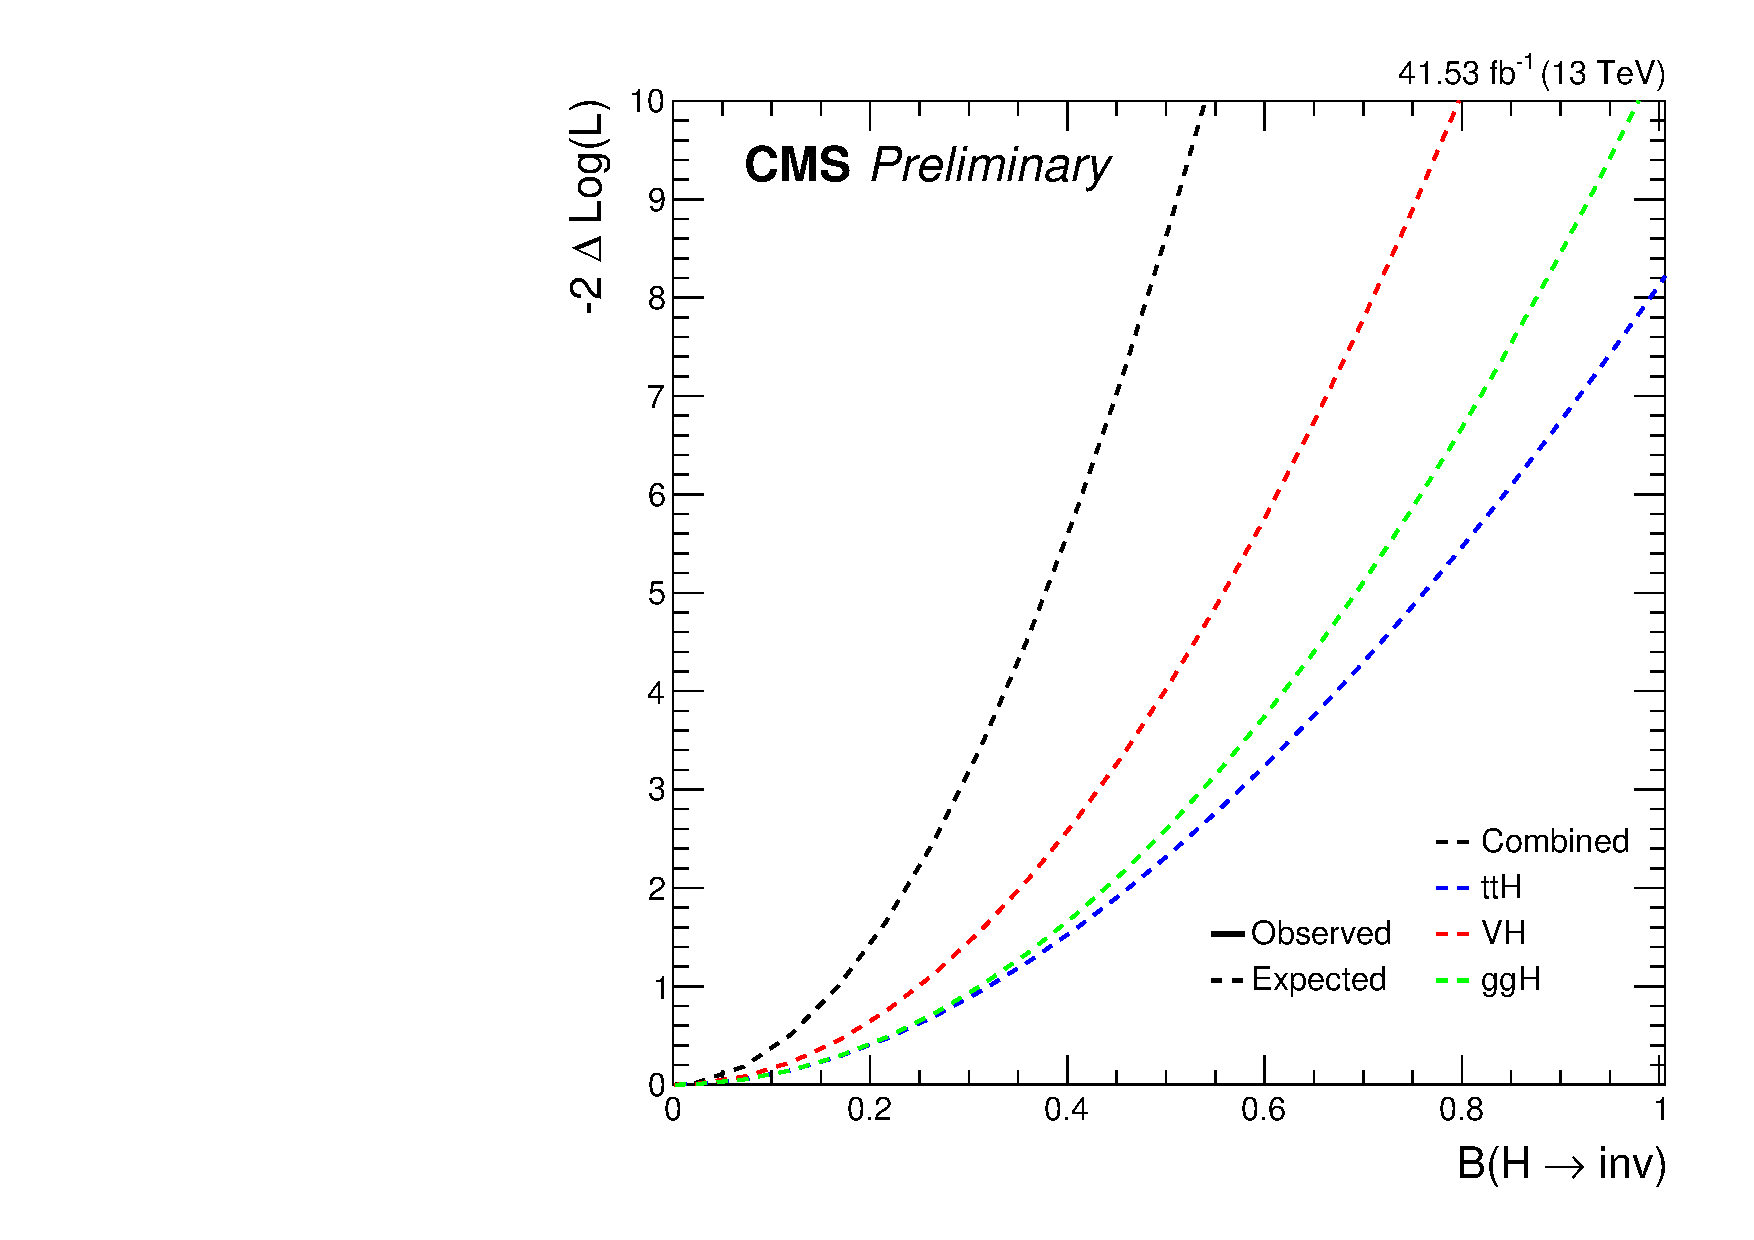
\includegraphics[width=\textwidth]{figures/likelihood_scan/profile_likelihood_scan_2017_Scenario5.pdf}
        \caption{Profile likelihood -- 2017}
    \end{subfigure}
    \caption[Expected 95\,\% CL upper limit on the Higgs boson to invisible state branching fraction $\BRof{\higgstoinv}$ and the corresponding profile likelihood ratio as a function of it, for both the individual categories that target a specific production mode, as well as the combination of them, for the 2017 dataset]{Expected 95\,\% CL upper limit on the Higgs boson to invisible state branching fraction $\BRof{\higgstoinv}$ (left) and the corresponding profile likelihood ratio as a function of it (right), for both the individual categories that target a specific production mode, as well as the combination of them, for the 2017 dataset. The \acrlong{sm} Higgs boson with its associated mass and production cross section are assumed.}
    \label{fig:htoinv_limit_likelihood_2017}
\end{figure}

\begin{figure}[htbp]
    \centering
    \begin{subfigure}[t]{0.45\textwidth}
        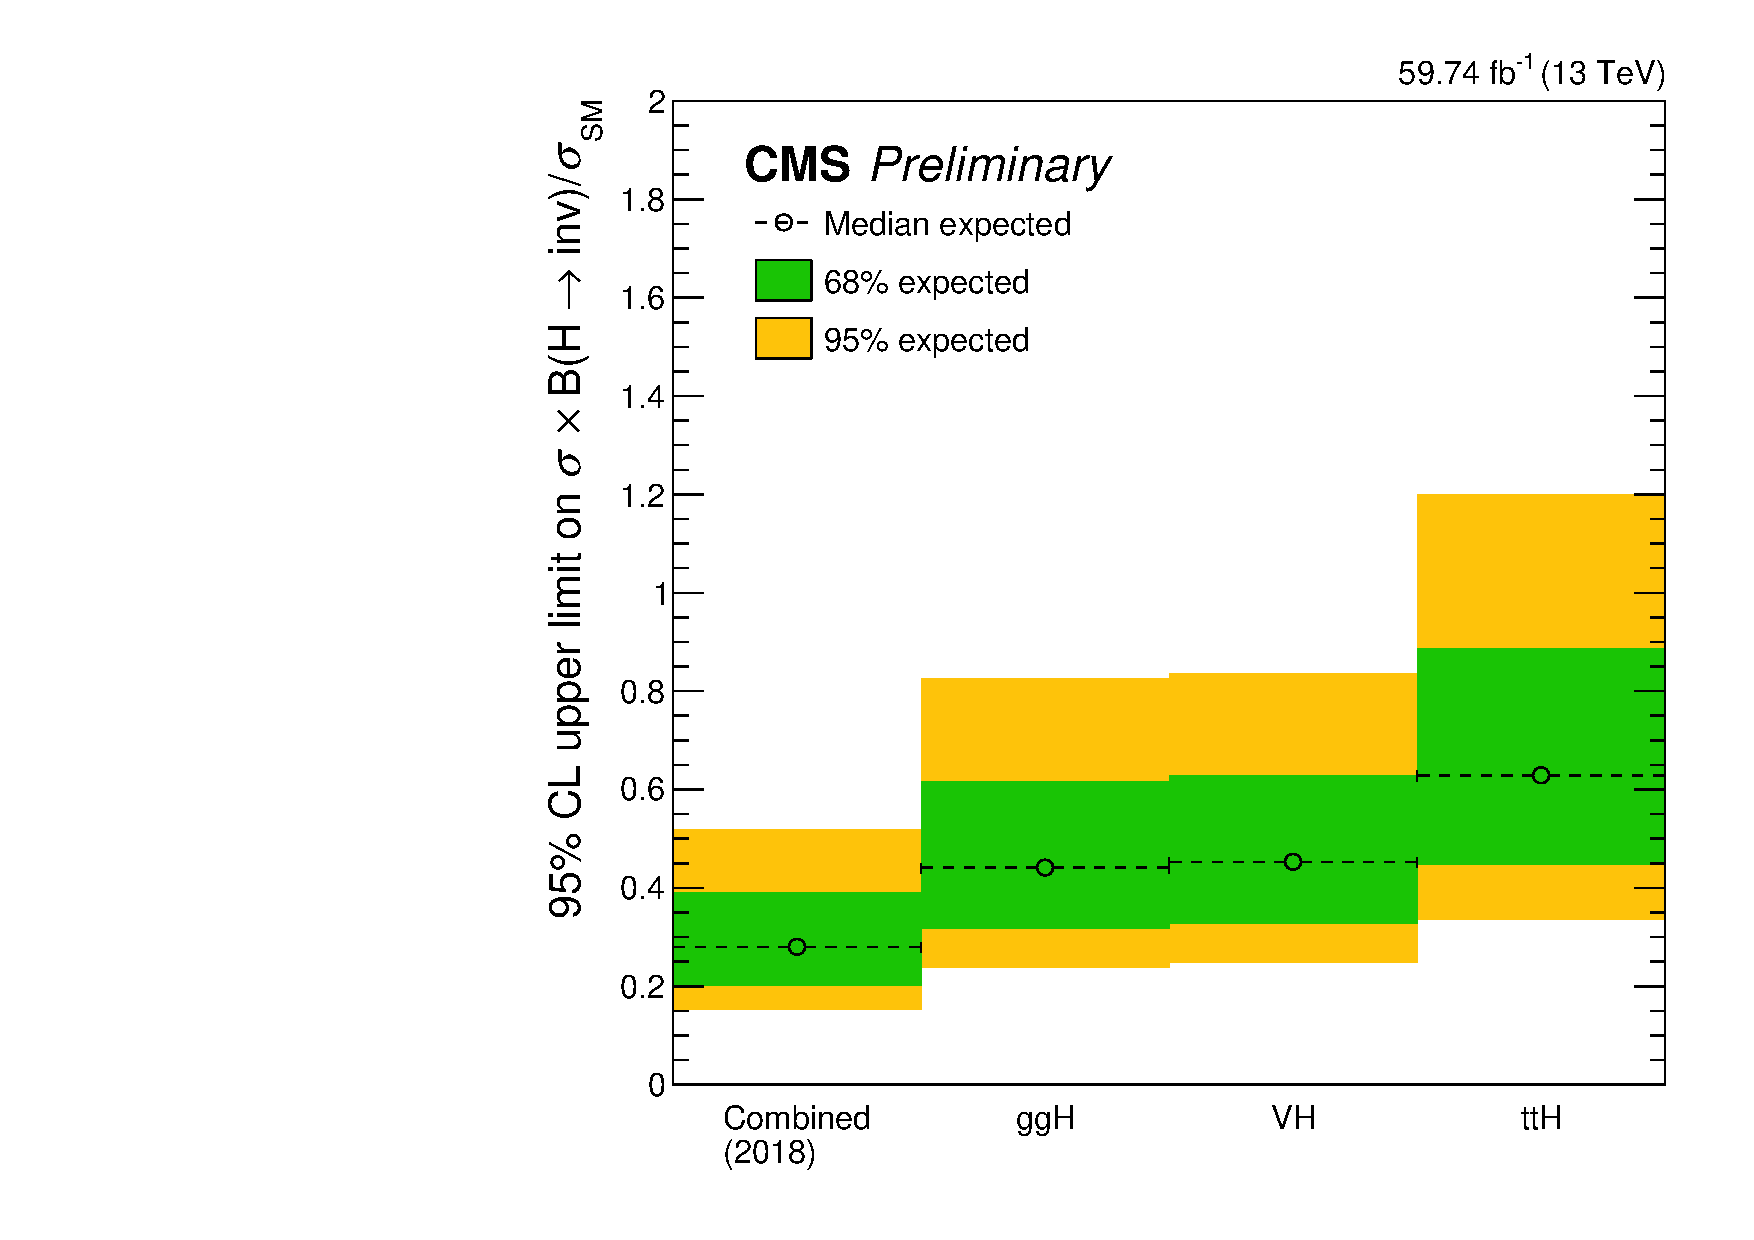
\includegraphics[width=\textwidth]{figures/limits/per_year/limit_2018_comb_Scenario5.pdf}
        \caption{Expected limit -- 2018}
    \end{subfigure}
    \hspace{0.05\textwidth}
    \begin{subfigure}[t]{0.45\textwidth}
        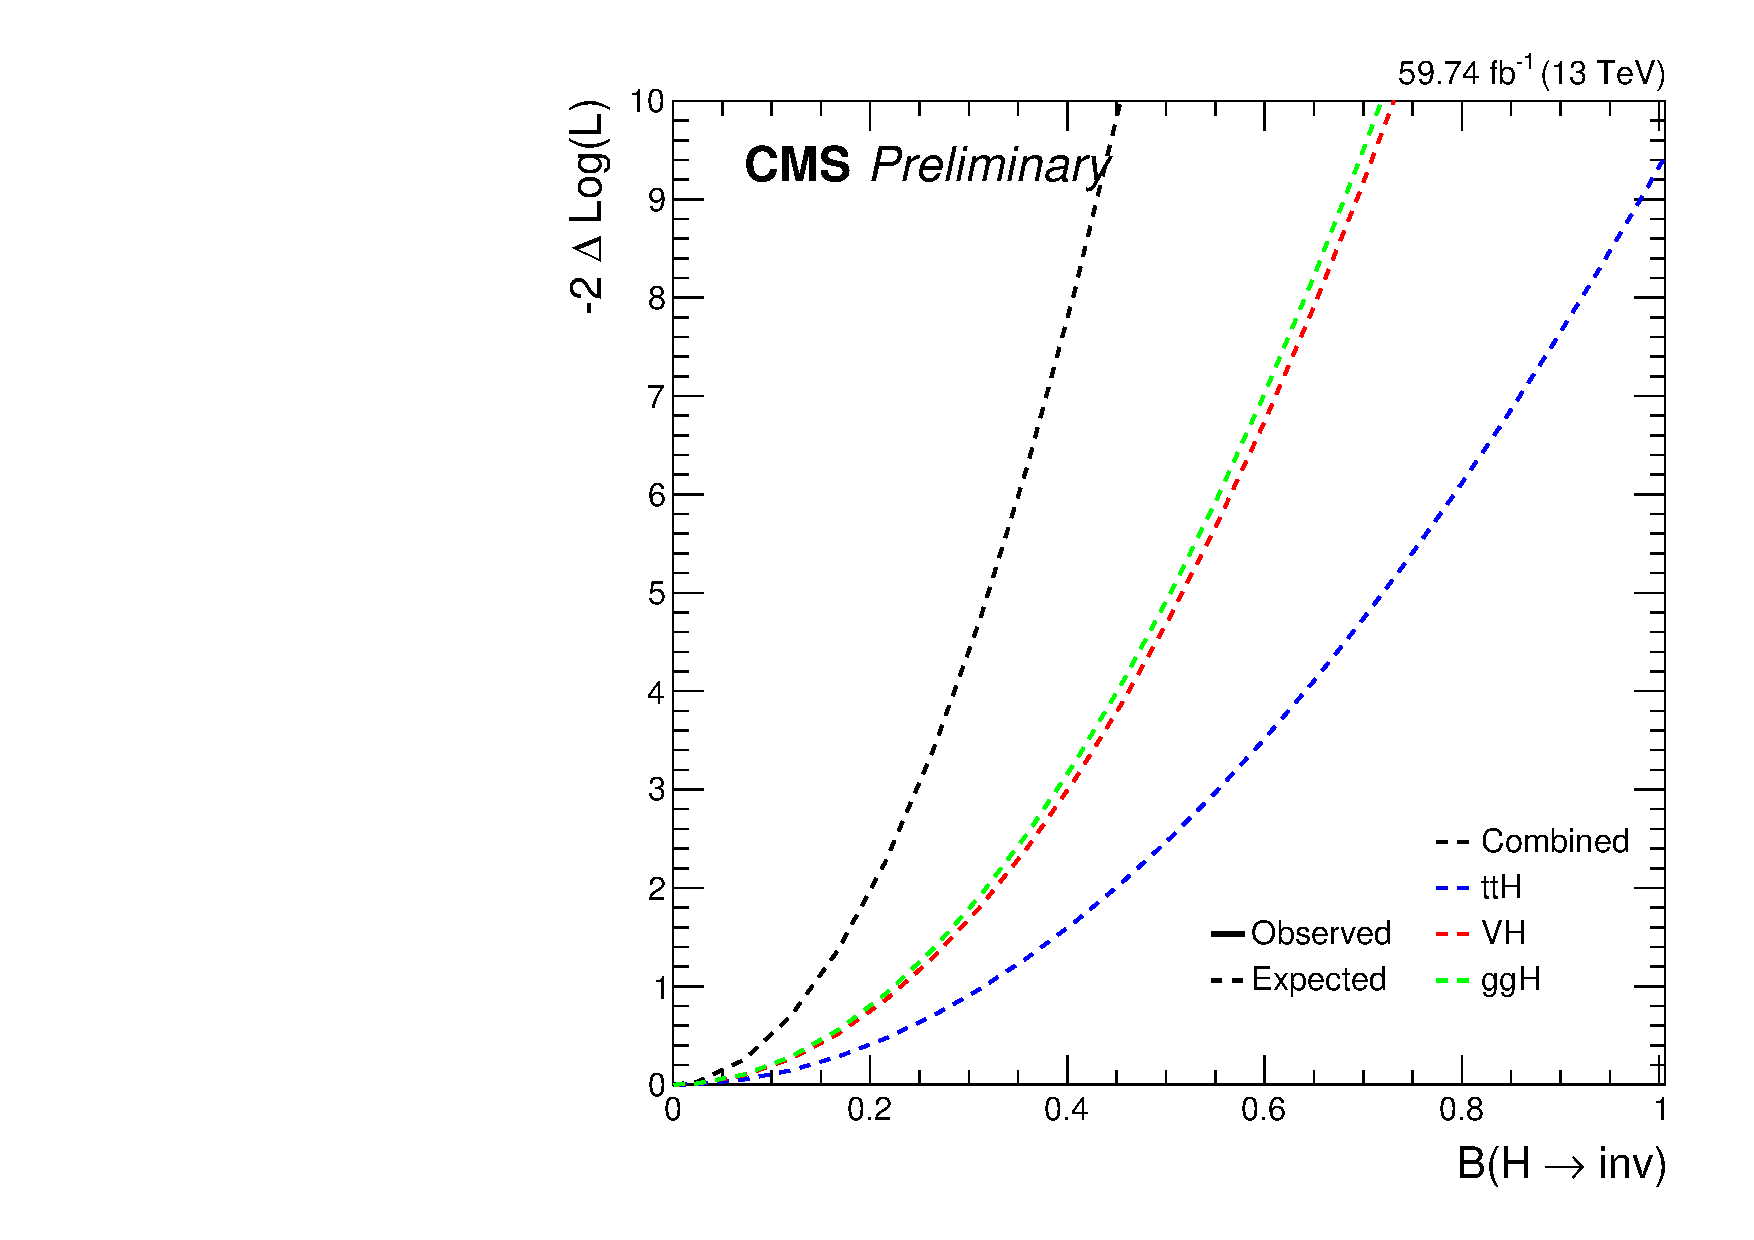
\includegraphics[width=\textwidth]{figures/likelihood_scan/profile_likelihood_scan_2018_Scenario5.pdf}
        \caption{Profile likelihood -- 2018}
    \end{subfigure}
    \caption[Expected 95\,\% CL upper limit on the Higgs boson to invisible state branching fraction $\BRof{\higgstoinv}$ and the corresponding profile likelihood ratio as a function of it, for both the individual categories that target a specific production mode, as well as the combination of them, for the 2018 dataset]{Expected 95\,\% CL upper limit on the Higgs boson to invisible state branching fraction $\BRof{\higgstoinv}$ (left) and the corresponding profile likelihood ratio as a function of it (right), for both the individual categories that target a specific production mode, as well as the combination of them, for the 2018 dataset. The \acrlong{sm} Higgs boson with its associated mass and production cross section are assumed.}
    \label{fig:htoinv_limit_likelihood_2018}
\end{figure}

\begin{figure}[htbp]
    \centering
    \begin{subfigure}[t]{0.45\textwidth}
        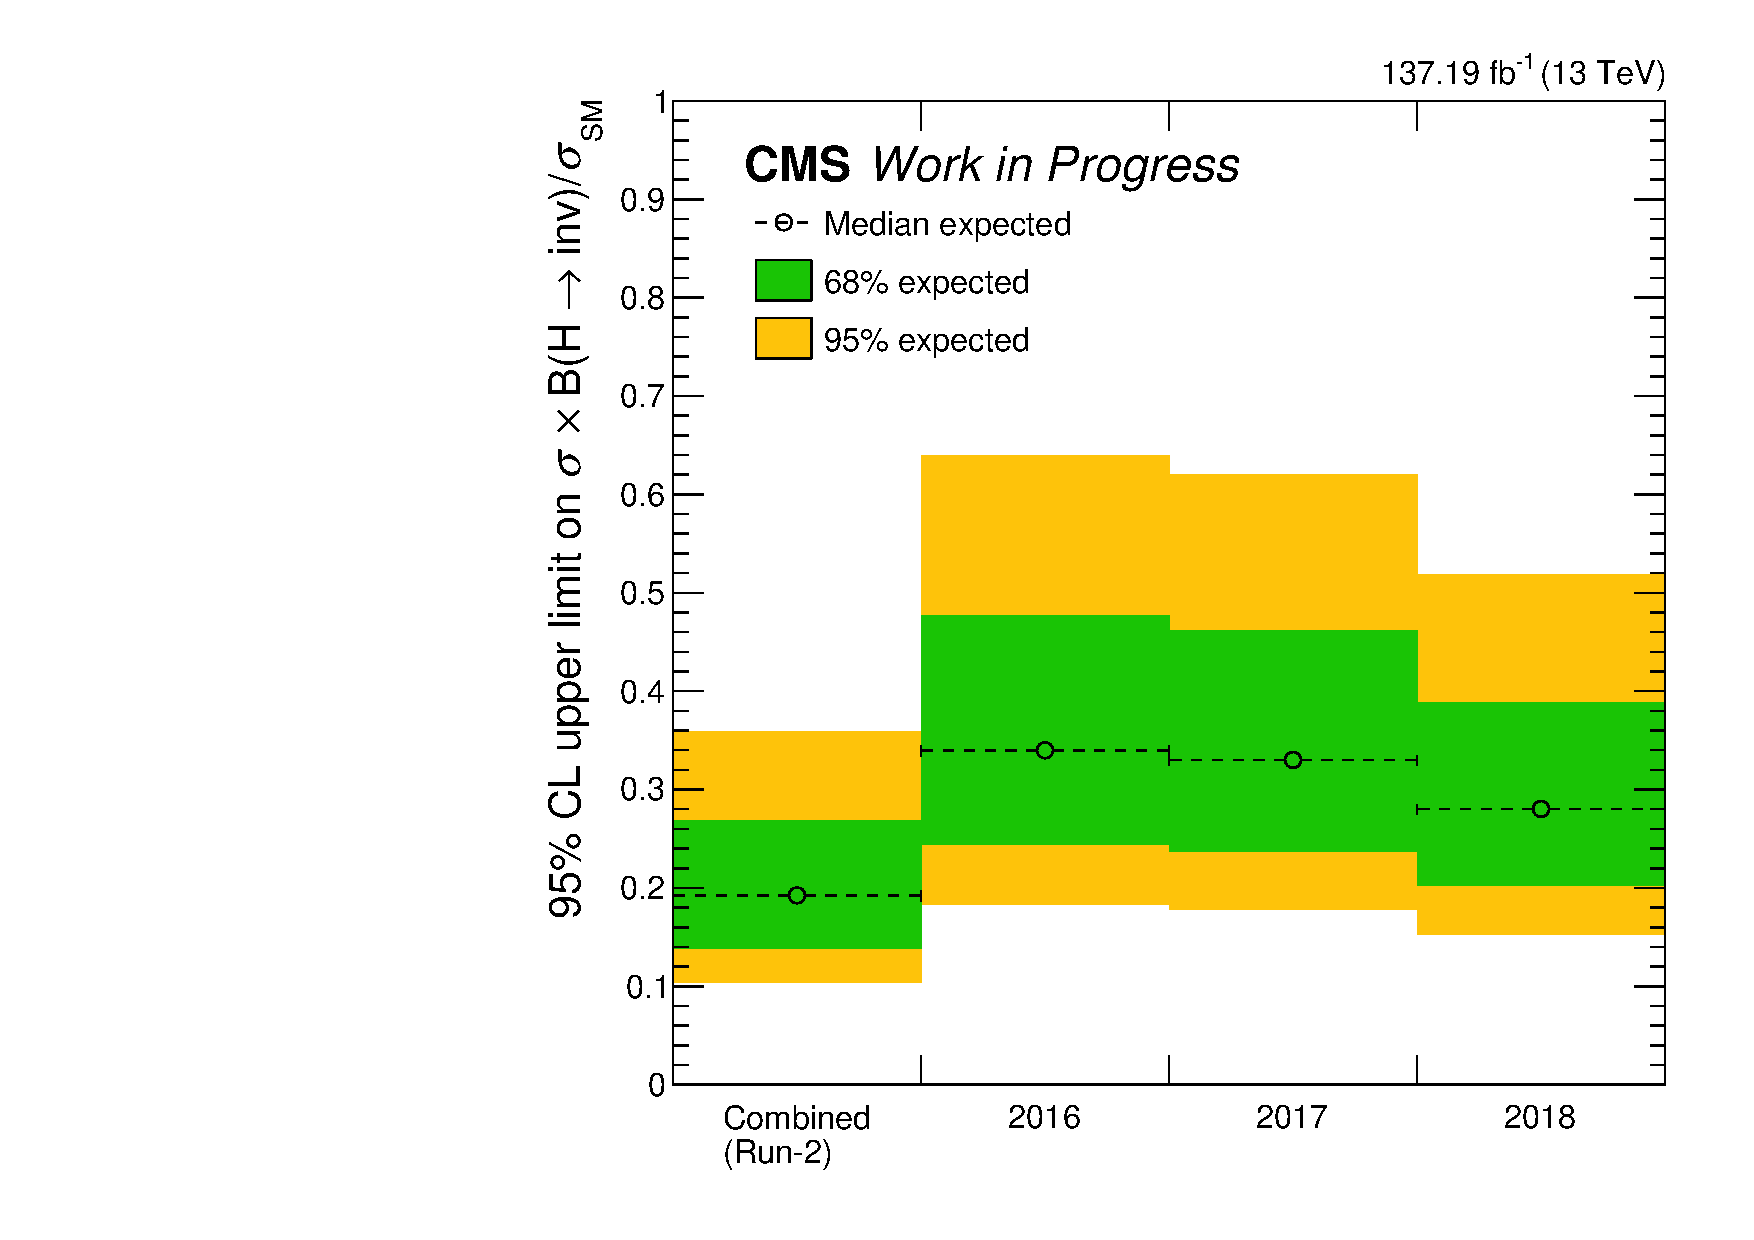
\includegraphics[width=\textwidth]{figures/limits/full_Run2/limit_Run2_comb_per_year_Scenario5.pdf}
        \caption{Expected limit -- Run-2}
    \end{subfigure}
    \hspace{0.05\textwidth}
    \begin{subfigure}[t]{0.45\textwidth}
        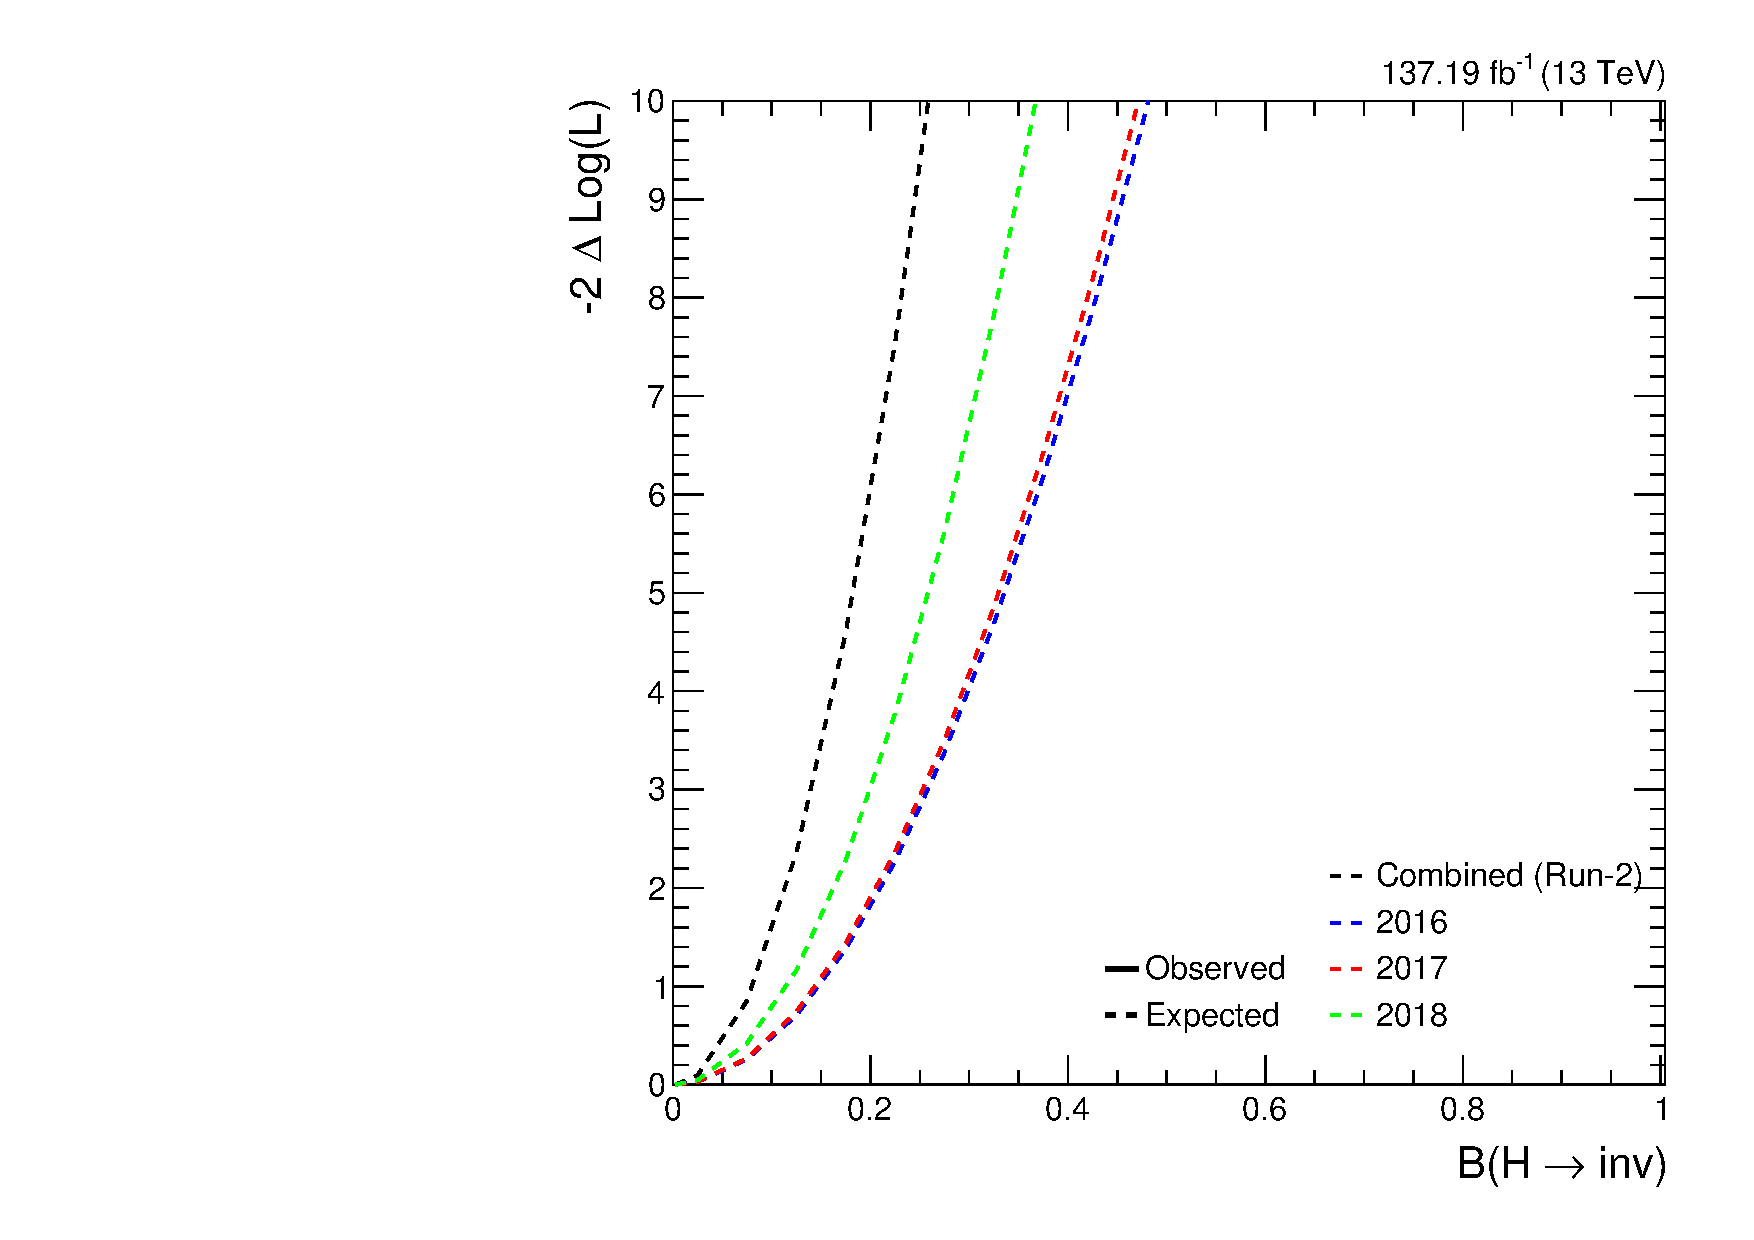
\includegraphics[width=\textwidth]{figures/likelihood_scan/profile_likelihood_scan_Run2_per_year_Scenario5.pdf}
        \caption{Profile likelihood -- Run-2}
    \end{subfigure}
    \caption[Expected 95\,\% CL upper limit on the Higgs boson to invisible state branching fraction $\BRof{\higgstoinv}$ and the corresponding profile likelihood ratio as a function of it, for both the individual data taking years, as well as the combination of them, for the full Run-2 dataset]{Expected 95\,\% CL upper limit on the Higgs boson to invisible state branching fraction $\BRof{\higgstoinv}$ (left) and the corresponding profile likelihood ratio as a function of it (right), for both the individual data taking years, as well as the combination of them, for the full Run-2 dataset. The \acrlong{sm} Higgs boson with its associated mass and production cross section are assumed.}
    \label{fig:htoinv_limit_likelihood_Run2_per_year}
\end{figure}

\begin{figure}[htbp]
    \centering
    \begin{subfigure}[b]{0.45\textwidth}  % top align since axis labels are larger for likelihood
        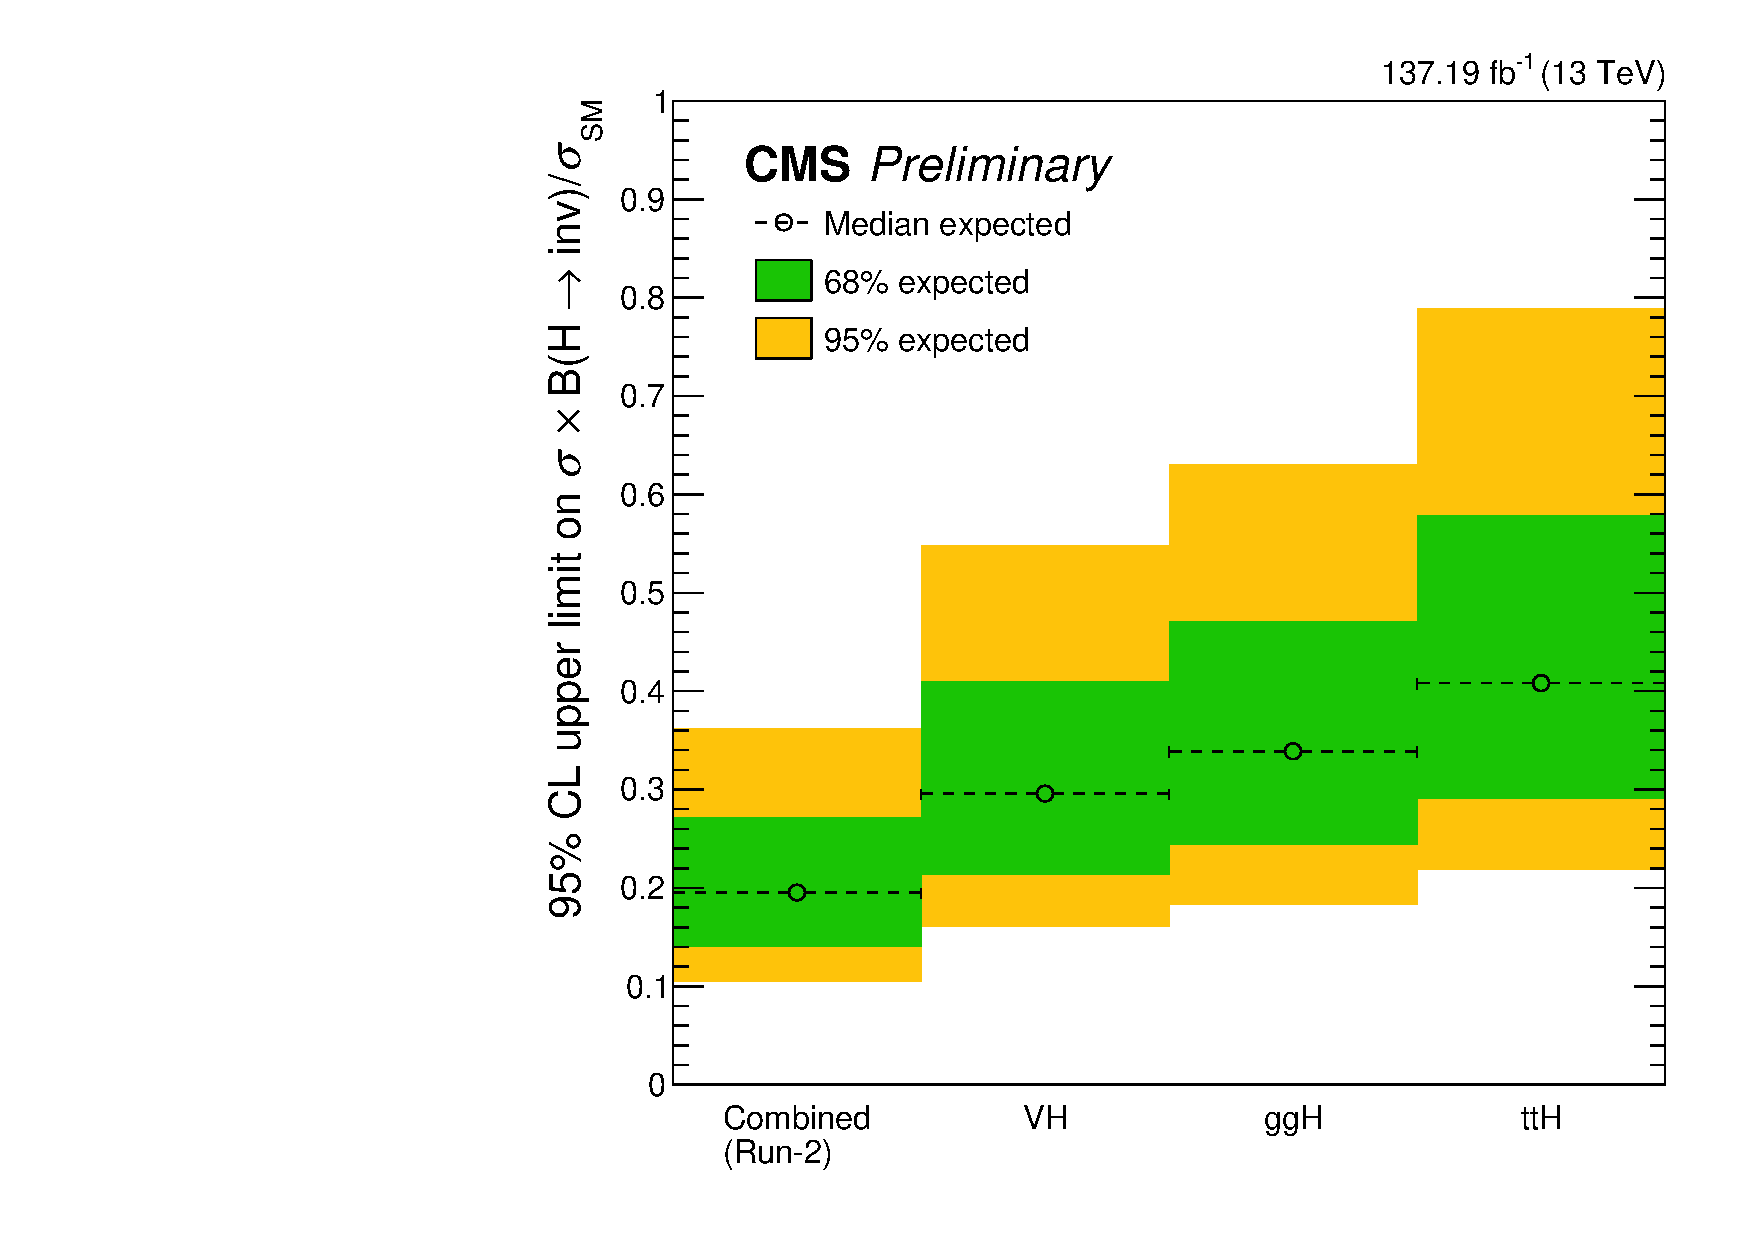
\includegraphics[width=\textwidth]{figures/limits/full_Run2/limit_Run2_comb_per_cat_Scenario5.pdf}
        \caption{Expected limit -- Run-2}
    \end{subfigure}
    \hspace{0.05\textwidth}
    \begin{subfigure}[b]{0.45\textwidth}
        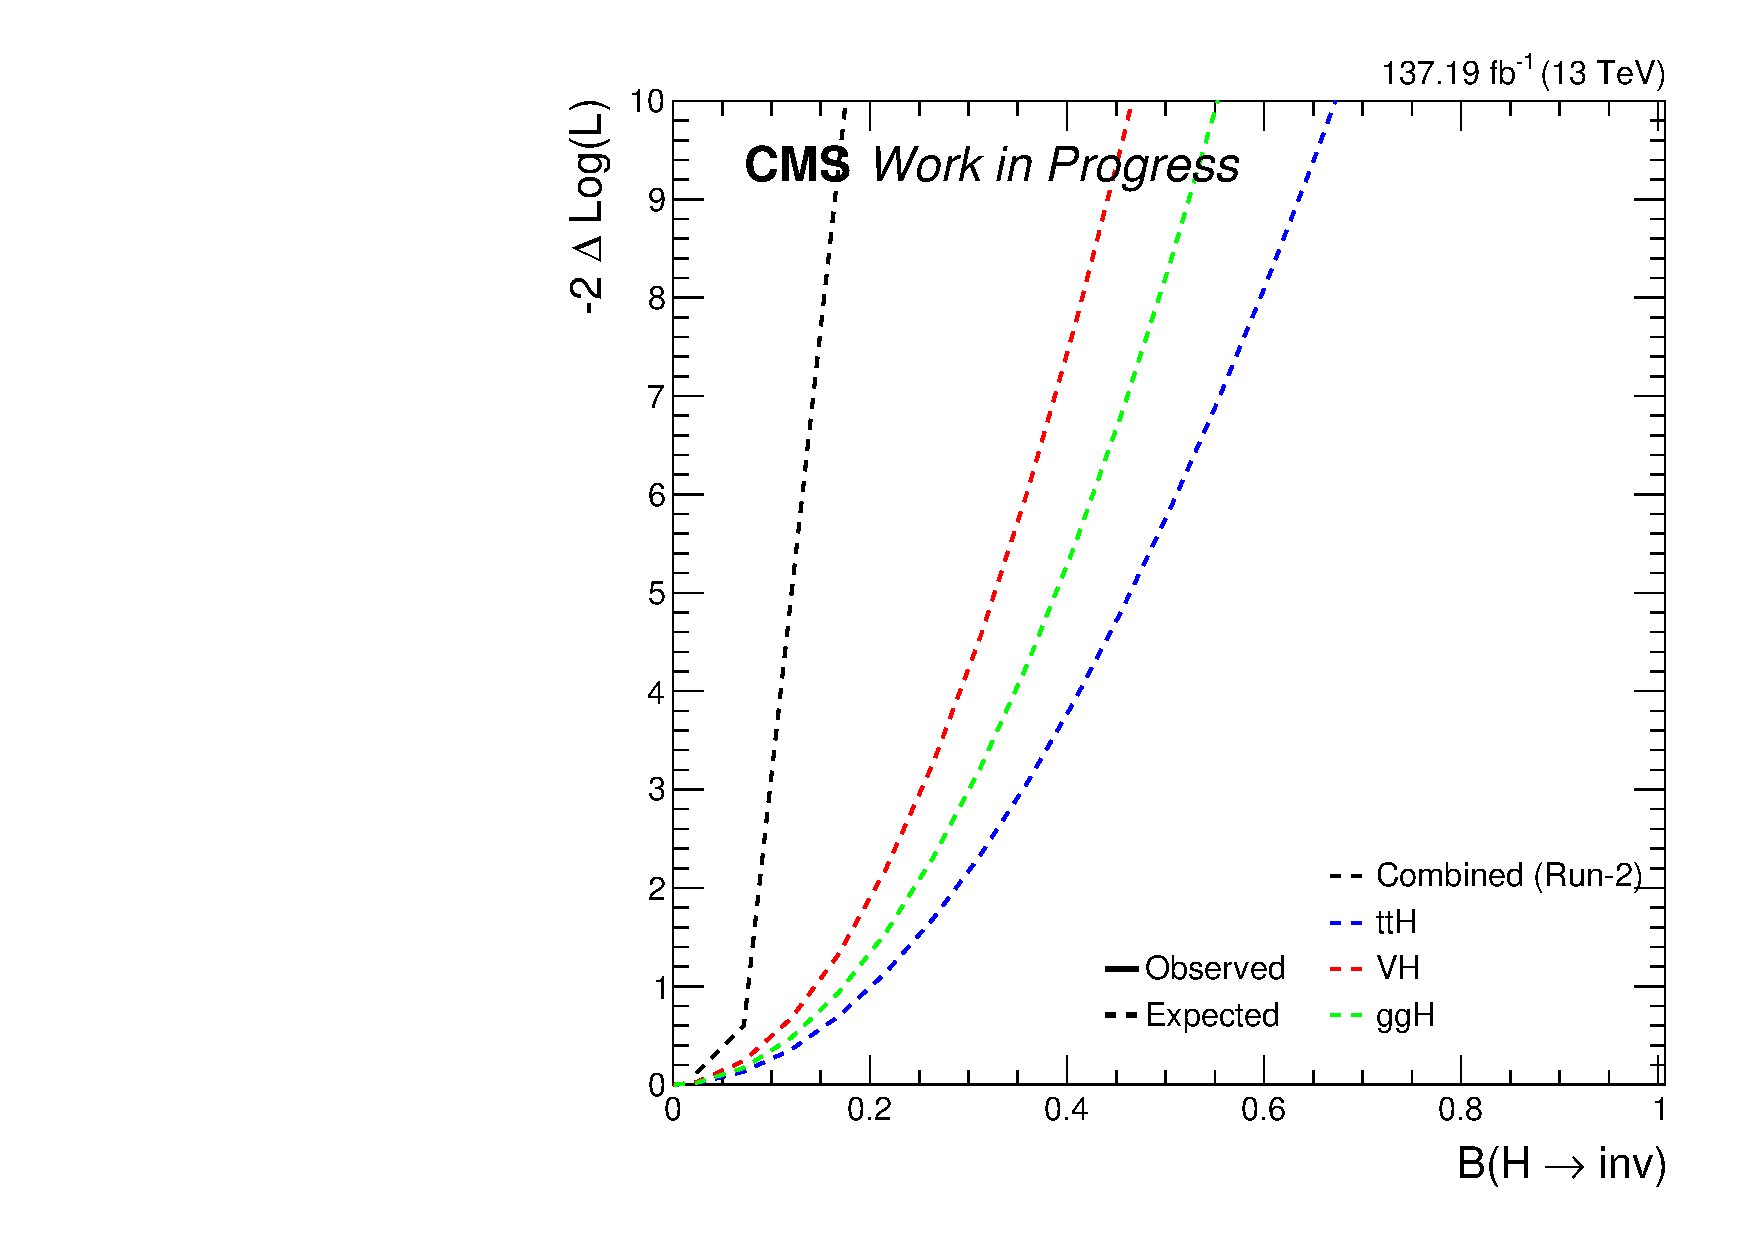
\includegraphics[width=\textwidth]{figures/likelihood_scan/profile_likelihood_scan_Run2_per_cat_Scenario5.pdf}
        \caption{Profile likelihood -- Run-2}
    \end{subfigure}
    \caption[Expected 95\,\% CL upper limit on the Higgs boson to invisible state branching fraction $\BRof{\higgstoinv}$ and the corresponding profile likelihood ratio as a function of it, for both the individual categories, as well as the combination of them, for the full Run-2 dataset]{Expected 95\,\% CL upper limit on the Higgs boson to invisible state branching fraction $\BRof{\higgstoinv}$ (left) and the corresponding profile likelihood ratio as a function of it (right), for both the individual categories, as well as the combination of them, for the full Run-2 dataset. The \acrlong{sm} Higgs boson with its associated mass and production cross section are assumed.}
    \label{fig:htoinv_limit_likelihood_Run2_per_cat}
\end{figure}

% Expected limits and likelihoods only, for Scenario 5. Have plots with VBF, but not combined with them. All limit and likelihood plots from 13th August


%=========================================================


\section{Interpretations in simplified dark matter scenarios}
\label{sec:htoinv_dark_matter_models}

The results of the analysis fail to accurately constrain the branching ratio on the Higgs boson to invisible state decays, with a value XXX times that of the \acrlong{sm} and no observation of the process. However, limits on certain properties of dark matter may be set. Two \acrshort{bsm} interpretations are presented: a Higgs portal model where the \acrshort{sm} acts as the mediator, and the existence of an additional, invisibly decaying, \acrshort{sm}-like Higgs boson.


%=========================================================


\subsection{Higgs portal model with the standard model Higgs boson}
\label{subsec:htoinv_dark_matter_higgs_portal}

One interpretation of our results may be in terms of a simplified Higgs portal model---coupling the dark sector to the visible where the \acrshort{sm} Higgs boson acts as the mediator bridging them. An effective field theory approach assumes that the invisible decays of the Higgs boson results in the pair production of dark matter particles \Pqdark, with a frequency constrained by the upper limit on $\BRof{\higgstoinv}$. If $\mqdark < m_{\PH}/\text{2}$, on-shell production allows the translation of the \higgstoinv width $\Gamma_{\mathrm{inv.}}$ into the spin-independent $\Pqdark$-nucleon scattering cross section \xsecSI, as in Ref.~\citenum{Djouadi:2011aa}. The interaction between dark and baryonic matter may be mediated by a Higgs boson, making direct detection experiments particularly sensitive to the recoil. The sensitivity of these experiments is typically parametrised by \xsecSI as a function of dark matter mass $\mqdark$. Comparisons can therefore be made between direct detection and collider experiments.

In this Higgs portal model, two cases are considered: the dark matter candidate is a scalar, or a Majorana fermion. The branching ratio is $\BRof{\higgstoinv} = \Gamma_{\mathrm{inv.}}/(\Gamma_{\mathrm{SM}} + \Gamma_{\mathrm{inv.}})$, where we assume $\Gamma_{\mathrm{SM}} = \text{4.07}\MeV$~\cite{Heinemeyer:1559921}. From Ref.~\citenum{Djouadi:2011aa}, $\Gamma_{\mathrm{inv.}}$ can be calculated for scalar $\Pqdark_{S}$ and fermion dark matter $\Pqdark_{f}$ as
\begin{equation}
    \begin{aligned}
\Gamma^{\mathrm{inv.}}_{\PH \rightarrow \Pqdark_{S}\Pqdark_{S}} &= \frac{ \lambda^2_{\PH SS} v^2 \beta_S }{64\pi m_{\PH}},\\[0.5em]
\Gamma^{\mathrm{inv.}}_{\PH \rightarrow \Pqdark_{f}\Pqdark_{f}} &= \frac{ \lambda^2_{\PH ff} v^2 m_{\PH} \beta_f^3 }{ 32\pi \Lambda^2 }
    \end{aligned}
\end{equation}

where $\lambda$ is the coupling (scaled by $\Lambda$ in the case of fermions)\footnote{Is $\Lambda$ some sort of scale, similar to $\Lambda_{\mathrm{QCD}}$?}, $v$ is the vacuum expectation value of the \acrshort{sm} Higgs field, and $\beta_i = \sqrt{1 - 4m_{\Pqdark_i}^2/m_{\PH}^2}$. The masses of the dark matter particles $mqdark$ are the physical masses after electroweak symmetry breaking with this new Higgs field. The spin-independent $\Pqdark$-nucleon scattering cross sections are
\begin{equation}
    \begin{aligned}
\sigma^{\mathrm{SI}}_{\Pqdark_{S}-N} &= \frac{\lambda^2_{\PH SS} }{ 16 \pi m_{\PH}^4} \frac{ m_N^4 f_N^2 }{ (m_{\Pqdark_{S}} + m_N)^2 },\\[0.5em]
\sigma^{\mathrm{SI}}_{\Pqdark_{f}-N} &= \frac{\lambda^2_{\PH ff} }{ 4 \pi \Lambda^2 m_{\PH}^4} \frac{ m_N^4 m_{\Pqdark_{f}}^2 f_N^2 }{ (m_{\Pqdark_{f}} + m_N)^2 }
    \end{aligned}
\end{equation}

where $f_N$ parametrises the Higgs-nucleon coupling. The value $f_N = \text{0.308} \pm \text{0.018}$ is taken from Ref.~\citenum{Hoferichter:2017olk}, recommended over that proposed in Ref.~\citenum{Djouadi:2011aa}. Limits on these cross sections as a function of dark matter mass are displayed in Fig.~\ref{fig:higgs_portal_dm_limits},\footnote{The plot is a placeholder for now, since we don't have final non-VBF/combined limits.} computed at 90\,\% confidence level to compare with direct detection experiments, whose latest results are also presented.

\begin{figure}
    \centering
    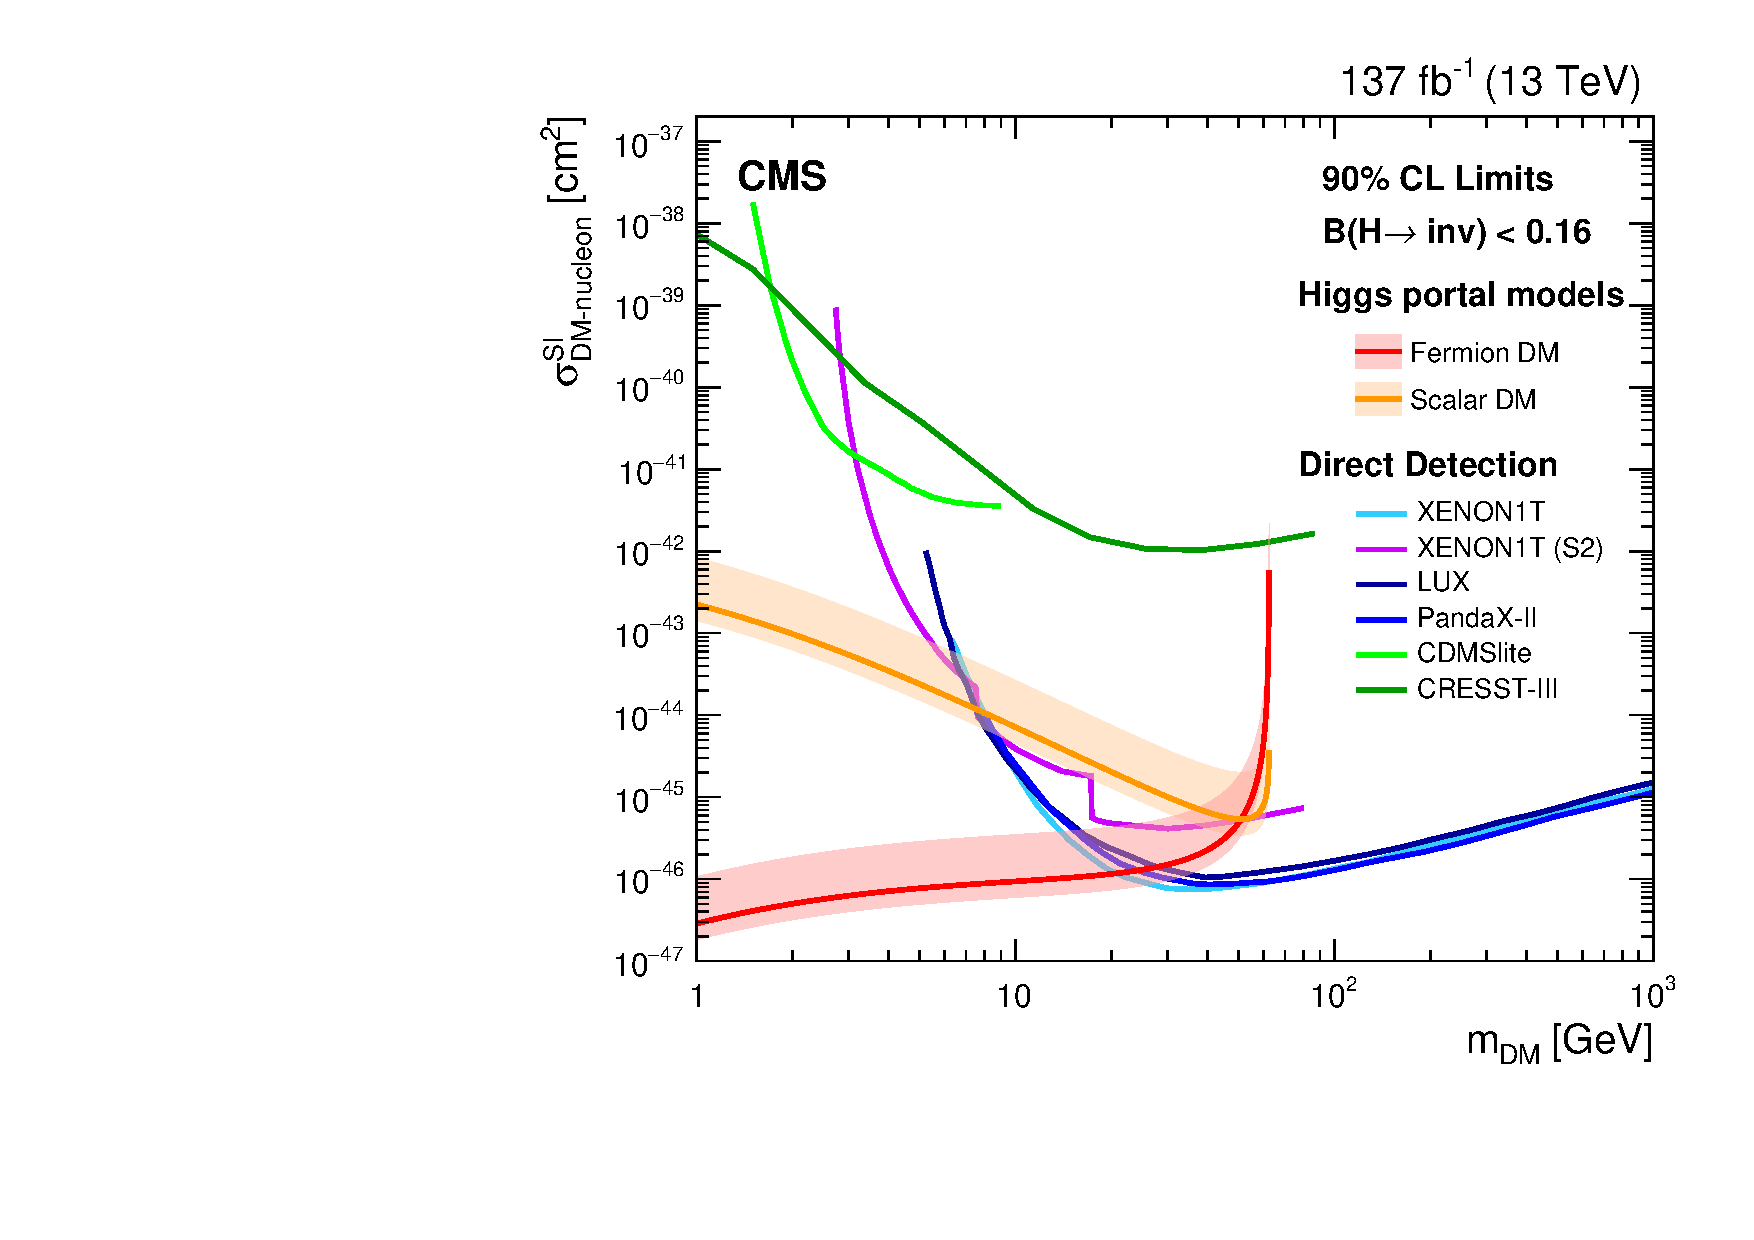
\includegraphics[width=0.5\textwidth]{figures/dark_matter_limit/higgsPortalDM.pdf}
    \caption[90\,\% confidence level upper limits on the spin-independent dark matter-nucleon scattering cross section in Higgs portal models, where the standard model Higgs boson decays into a pair of scalar (solid orange) or fermion (dashed red) dark matter particles]{90\,\% confidence level upper limits on the spin-independent dark matter-nucleon scattering cross section in Higgs portal models, where the \acrlong{sm} Higgs boson decays into a pair of scalar (solid orange) or fermion (dashed red) dark matter particles. Comparisons to direct detection experiments are also provided: XENON1T~\cite{Aprile:2018dbl} (additionally with the S2-only analysis~\cite{Aprile:2019xxb}), LUX~\cite{Akerib:2016vxi}, PandaX-II~\cite{Cui:2017nnn}, CDMSlite~\cite{Agnese:2018gze}, and CRESST-III~\cite{Abdelhameed:2019hmk}.}
    \label{fig:higgs_portal_dm_limits}
\end{figure}

For $\BRof{\higgstoinv} < XX$, the Higgs portal models assuming scalar and fermion dark matter candidates set the lowest limits on \xsecSI for \mqdark below Y and Z\GeV, respectively.

% Potentially also include the kappa_v, kappa_f plot, and discuss


%=========================================================


\subsection{Constraints on a standard model-like Higgs boson}
\label{subsec:htoinv_dark_matter_bsm_higgs}

If the \acrshort{sm} Higgs boson does not decay into invisible particles beside the neutrino, one may still hypothesize a scenario in which the Higgs field is associated with dark matter. The next-to-minimal branch of \acrlong{susy} and models with two Higgs doublets are examples that accommodate an additional Higgs boson with a different mass that does not couple to the \acrshort{sm} variant. It is denoted as ``\acrlong{sm}-like,'' since it may be produced via the same mechanisms as the \acrshort{sm} Higgs boson (\ttH, \VH, \ggH, and \acrshort{vbf}) with the same relative contributions from each one. This extra Higgs is assumed to decay exclusively to invisible states.

We perform our analysis where we assume an additional Higgs boson, and show the limit on the branching ratio as a function of mass.

% This subsection should discuss analysis of signal samples with non-Standard Model Higgs masses. Some useful info on those: https://twiki.cern.ch/twiki/bin/view/LHCPhysics/CERNYellowReportPageBSMAt13TeV
